% Releases:
% Version 0.0 for Hobbes 0.4.0.0-r38

\documentclass[12pt,letterpaper]{article}
\usepackage[utf8x]{inputenc}
\usepackage[normalem]{ulem}
\usepackage{ucs}
\usepackage{amsmath}
\usepackage{amsfonts}
\usepackage{amssymb}
\usepackage[pdftex]{graphicx}
\usepackage[margin=1in]{geometry}
\usepackage{hyperref}
\usepackage{color}
\usepackage{listings}
\usepackage[scaled=0.81]{inconsolata}
\setcounter{secnumdepth}{5}
\setcounter{tocdepth}{5}

\definecolor{green}{RGB}{0,176,80}
\definecolor{lightgreen}{RGB}{148,208,80}
\definecolor{red}{RGB}{255,0,0}
\definecolor{lightpurple}{RGB}{191,177,207}
\definecolor{purple}{RGB}{146,122,173}
\definecolor{blue}{RGB}{52,117,205}
\definecolor{orange}{RGB}{217,104,13}
\definecolor{white}{RGB}{255,255,255}

\lstset{language=Python}
\lstset{showstringspaces=false}

\author{Angus Lim}
\begin{document}

\begin{center}

\huge The Hobbes Design Document \\ \large Version 0.0

\end{center}

\tableofcontents
\pagebreak

\setcounter{section}{-1}



%
% Section 0
%
\section{Introduction}
\label{0}

\textbf{Hobbes} is an application that communicates with a target via a serial port, where the target is presumably an Icron board. At the most basic level, Hobbes is capable of sending commands and firmware to the target, and receiving messages from it.

\setcounter{subsection}{-1}



%
% Section 0.0
%
\subsection{Purpose}
\label{0.0}

The purpose of this document is to describe the design and functionality of Hobbes.



%
% Section 0.1
%
\subsection{Scope}
\label{0.1}

This document will mostly concern the design of Hobbes. A somewhat abstract view of Hobbes will be taken to allow a variety of implementations. As Hobbes is currently written in IronPython, though, many examples will be given in that language.



%
% Section 0.2
%
\subsection{Terminology References}
\label{0.2}

\begin{itemize}

\item Hobbes: the program itself

\item Hobbes 0: the current implementation of Hobbes in IronPython

\item Calvin: the Python interpreter running in Hobbes

\item LG1: Lionsgate project

\item GE: Goldenears project

\item XML: Extensible Markup Language

\item JSON: JavaScript Object Notation

\end{itemize}



%
% Section 0.3
%
\subsection{Document References}
\label{0.3}

The only real references here are the \href{http://docs.python.org/library/}{Python standard library} and the \href{http://msdn.microsoft.com/en-us/library/gg145045.aspx}{.NET library}.



%
% Section 1
%
\section{Design Overview}
\label{1}

\setcounter{subsection}{-1}



%
% Section 1.0
%
\subsection{Background Information}
\label{1.0}

This document is about the design of Hobbes, hence the name of this document being ``The Hobbes Design Document''. One wishing only to learn how to use Hobbes should not read this document; the User's Guide is provided for that purpose. This document is better suited towards one that wishes to modify, improve, or even completely rewrite, Hobbes.



%
% Section 1.1
%
\subsection{System Evolution Description}
\label{1.1}

By no means is Hobbes complete. By no means is it completely stable. There are a bunch of things that can be improved:

\begin{itemize}

\item Ongoing GUI improvements. There will probably always be some seemingly tedious task that can be simplified by the addition of a button/checkbox/etc. There is a trade-off in speed, though.

\item Other projects. At the moment, anything other than LG1 and GE is not supported well in Hobbes.

\item Other file transfer protocols. Although unlikely, Hobbes may need to support things other than Stewie and XMODEM in the future.

\item Saving data. Currently, Hobbes uses a mix of XML and JSON to store and load data. JSON is just as readable as XML and is much more lightweight, so XML should be phased out.

\item Porting Hobbes to a different language. Hobbes is currently implemented in IronPython, a flavour of Python that allows easy integration with the .NET Framework. Although this is useful (basically having two completely difference libraries available), it's a bit awkward; it also doesn't help that I was lazy in some parts of Hobbes by copying Tigger code and correcting the syntax (e.g. when running bsdtar.exe on a .icron file). In addition, Windows is apparently terrible at serial port communication, so that may have a hand in Hobbes occasionally freezing when receiving a ton of bytes.

If Hobbes is ported, it should be to CPython. Certainly, it would be the easiest to port to; with the \href{http://pyserial.sourceforge.net/}{pySerial module}, serial port communication can be accomplished with .NET. The Python standard library should be large enough to do everything else--for example, the \href{http://docs.python.org/library/bz2.html}{bz2 module} can replace bsdtar.exe and the whole Process/ProcessStartInfo thing in Tigger and Hobbes. The current GUI layer of Hobbes is written in IronPython, but calls all the System.Windows.Forms stuff in .NET; with a CPython-written Hobbes one could use Python 3, PyGObject, GTK+ 3, and Glade, which is probably better suited towards Linux development.

\end{itemize}



%
% Section 1.2
%
\subsection{Current Process}
\label{1.2}

The program to be phased out is Tigger, itself a replacement for an even older program named Leo. Basically, Tigger does everything Hobbes does, except a) for the most part slower and b) without any scripting capabilities.

Here's Tigger's process, from its own design document:

``The new process is also a C\# application which includes the capability of having multiple serial connections simultaneously allowing for simultaneous communication with multiple targets. The new solution also includes multiple protocols for programming a target, including binary flash, stewie and xmodem 1k. It also allows for different protocols for parsing data from a target, and currently parses using two protocols, the one included in the original Leo and the new ilog system.''



%
% Section 1.3
%
\subsection{User Characteristics}
\label{1.3}

\setcounter{subsubsection}{-1}



%
% Section 1.3.0
%
\subsubsection{User Problem Statement}
\label{1.3.0}

Basically, Hobbes was created in an (extremely successful, if I may say so myself) attempt to add a Python component to Tigger, adding a scripting capability to communication with Icron boards.



%
% Section 1.3.1
%
\subsubsection{User Objectives}
\label{1.3.1}

As Hobbes is a replacement for Tigger, its design will contain the objectives of Tigger:

\begin{itemize}

\item Easy to use

\item Convenient

\item Utilize a quick protocol for programming targets

\item Allow for multiple protocols for programming and logging, and enable easy inclusion of new protocols

\item Not crash frequently at all

\item Not cause user frustration and pain

\end{itemize}

\noindent In addition, Hobbes contains additional objectives for its scripting layer:

\begin{itemize}

\item Provide a functional Python (or other scripting language) interpreter

\item Allow scripts for said interpreter to be saved, loaded, and executed

\end{itemize}



%
% Section 1.4
%
\subsection{Proposed Process}
\label{1.4}

Software development since Tigger was released have resulted in many features of Tigger becoming obsolete. Some examples are XMODEM 1K, binary flash, a bunch of serial port options, and Leo-era logging. Hobbes strips these unnecessary components of Tigger away, and adds a command-line interpreter for scripting.



%
% Section 1.5
%
\subsection{Constraints}
\label{1.5}

Since Hobbes is currently implemented using the .NET Framework, it uses the SerialPort class for connection to serial ports, and thus presumably has the serial port disconnect issue that Tigger apparently had. Using PySerial and/or Linux may help.

GUI addons have slowed Hobbes's IronPython implementation down significantly; the biggest factor is probably an iLog setting the font and font colour of the output textbox when it's displayed, regardless of whether custom fonts are being used at all. In addition, scrolling and truncating text in the output textbox is somewhat awkward in .NET. Using a GtkTextBuffer in GTK+ (with GtkTextTag for custom fonts) would probably be easier.

In addition, the current interpreter is not quite at the level of a Python interpreter; that is, generally to see output one has to prefix a statement with ``print''. For example, while the input ``2 + 2'' would output 4 in a CPython/IronPython interpreter, Hobbes's interpreter will output nothing unless the input is ``print 2 + 2''.

%This section should mention all limitations, assumptions, and rules for using this design.

%This new design is currently constrained in it is save functionality as ini files instead of xml files are utilized.  There are also constraints imposed by a bug in the.Net framework serial port for which a workaround has been implemented.  This bug, if left unhandled, causes a crash when the UART is physically unplugged or the power to the ASIC is cycled. The workaround for this bug is composed of two parts, the first of which is the enabling legacy exception handling which catches and ignores the exception which causes the crash.  The second part of the workaround is to allow for quick serial reconnection during ASIC power cycling.  The serial port does not automatically reopen once the ASIC is cycled on, and so the workaround involves pressing a button, once the ASIC has been powered off, that tells tigger to listen for a connection to the ASIC to become available.  In this situation, tigger then listens for the connection to become avaialbe, and once it does it opens it.  Unfortunately, there is the potential for data to be lost, before tigger can recognize and reopen the connection. There are also currently constraints imposed by the target’s ability to receive many bytes at once, and so currently the binary flash is very slow.



%
% Section 1.6
%
\subsection{Design Trade-offs}
\label{1.6}

Generally, more GUI components means slower execution speed. Hobbes was originally designed to focus only on scripting; as development progressed, GUI components were added to satisfy the demands of the non-scripting user.



%
% Section 2
%
\section{Design Architecture}
\label{2}

\setcounter{subsection}{-1}



%
% Section 2.0
%
\subsection{HobbesDriver}
\label{2.0}

Does nothing more than create an instance of the HobbesInterpreter class and catches any exception, displaying an error window if one is raised. This code should be able to reside in HobbesInterpreter without any trouble, so implementing this module is somewhat optional.



%
% Section 2.1
%
\subsection{HobbesInterpreter}
\label{2.1}

User interaction through the console should take place in this module, as the Python engine Calvin is here. There is also a StartupWindow class that contains, well, a startup window.



%
% Section 2.2
%
\subsection{ErrorWindow}
\label{2.2}

Pops up (usually) when something bad happens. Writes information on the exception that was raised to an error log.



%
% Section 2.3
%
\subsection{Device}
\label{2.3}

Provides the actual connection to the serial port, so this is probably the most important module in Hobbes. The DeviceWindow class in this module allows input to Calvin, and prints iLog output from the serial port to a textbox. Any GUI components to aid user communication to/from the serial port is in this window.



%
% Section 2.4
%
\subsection{XMLSettings}
\label{2.4}

Uses XML to save and load settings for other modules. However, if Python is used, a dictionary or list should suffice, and JSON can be used to save settings to disk. As a result, this module should be deprecated.



%
% Section 2.5
%
\subsection{iCommand}
\label{2.5}

Provides facilities to write to the serial port, signifying a command to execute. Optionally contains an iCommandWindow class that allows the user to interactively select an iCommand to send or save to an alias.



%
% Section 2.6
%
\subsection{iLog}
\label{2.6}

Provides facilities to display iLogs received from the serial port. Optionally contains an iLogWindow class that allows the user to modify the font and colour used to display each individual iLog when it is received.



%
% Section 2.7
%
\subsection{iCmdResp}
\label{2.7}

Only useful for scripting users. Amalgamates an iCommand and iLog such that executing a function corresponding to an iCmdResp executes an iCommand, waits for a specific iLog to be received, parses a specific argument from said iLog, and returns the argument.



%
% Section 2.8
%
\subsection{Stewie}
\label{2.8}

Sends an image file to a board using the Stewie file transfer protocol.



%
% Section 2.9
%
\subsection{XMODEM}
\label{2.9}

Sends an image file to a board using the XMODEM file transfer protocol.



%
% Section 3
%
\section{External Module interface}
\label{3}

\setcounter{subsection}{-1}



%
% Section 3.0
%
\subsection{Use model}
\label{3.0}

There are sort of two layers to Hobbes:

\begin{itemize}

\item \emph{The ``Calvin and Hobbes'' layer.} In the current implementation of Hobbes, the instance of the HobbesInterpreter class being run is named ``hobbes'' and the actual Python engine is named ``Calvin''; hence the name. This layer consists solely of a command prompt and enough functions and variables to do anything to a Device. Note that iLogs automatically go to a window, so you won't see them if you purely work within the console.

\item \emph{The ``Watterson'' layer.} That is, the pretty GUI stuff. Note that Hobbes focusses on scripting, so clicking a button in a GUI component should in fact call a function in some code sent to the interpreter. GUIs are overrated. The GUI is should only be a convenience to the user; it should not be able to do anything that scripting cannot.

Hobbes 0 uses a function to execute code from a GUI that looks similar to this:

\fontfamily{fi4}\selectfont

\begin{lstlisting}
def execute_code():
    '''Executes code using a Python engine.'''
    # compile code, and attempt to execute
    source = python_engine.CreateScriptSourceFromString(
             python_code, SourceCodeKind.Statements)
    try:
        source.Execute(python_scope)
    except Exception as ex:
        # show the error that's occurred
        eo = python_engine.GetService[ExceptionOperations]()
        error = eo.FormatException(ex)
        MessageBox.Show(error)
\end{lstlisting}

\fontfamily{cmr}\selectfont

There are a few different implementations of this in Hobbes 0 to allow for different variables replacing ``python\_engine'', ``python\_scope'', and ``python\_code''. They all point to the same Python engine, scope, and code, though. And of course, a CPython implementation of Hobbes would have a totally different exception block.

\end{itemize}

%How is this design intended to be used?  For example is this by providing an API to call? Will it operate on a global state? Should the caller setup function pointers to be called back to? Or does this module configure itself with function pointers to be called?



%
% Section 3.1
%
\subsection{API/Data Structures}
\label{3.1}

See \hyperref[4]{$\S4$} for everything regarding APIs and data structures.



%
% Section 4
%
\section{Detailed Design}
\label{4}

The following diagram details the interaction between all the modules in Hobbes 0.

Here's a summary of each module first:

{
\color{green}
\hyperref[4.0]{HobbesDriver}
}

{
\color{green}
\hyperref[4.1]{HobbesInterpreter}
}

{
\color{red}
\hyperref[4.2]{ErrorWindow}
}

{
\color{green}
\hyperref[4.3]{Device}
}

{
\color{lightgreen}
\hyperref[4.4]{XMLSettings}
}

{
\color{purple}
\hyperref[4.5]{iCommand}
}

{
\color{purple}
\hyperref[4.6]{iLog}
}

{
\color{lightpurple}
\hyperref[4.7]{iCmdResp}
}

{
\color{blue}
\hyperref[4.8]{Stewie}
}

{
\color{blue}
\hyperref[4.9]{XMODEM}
}


\begin{center}
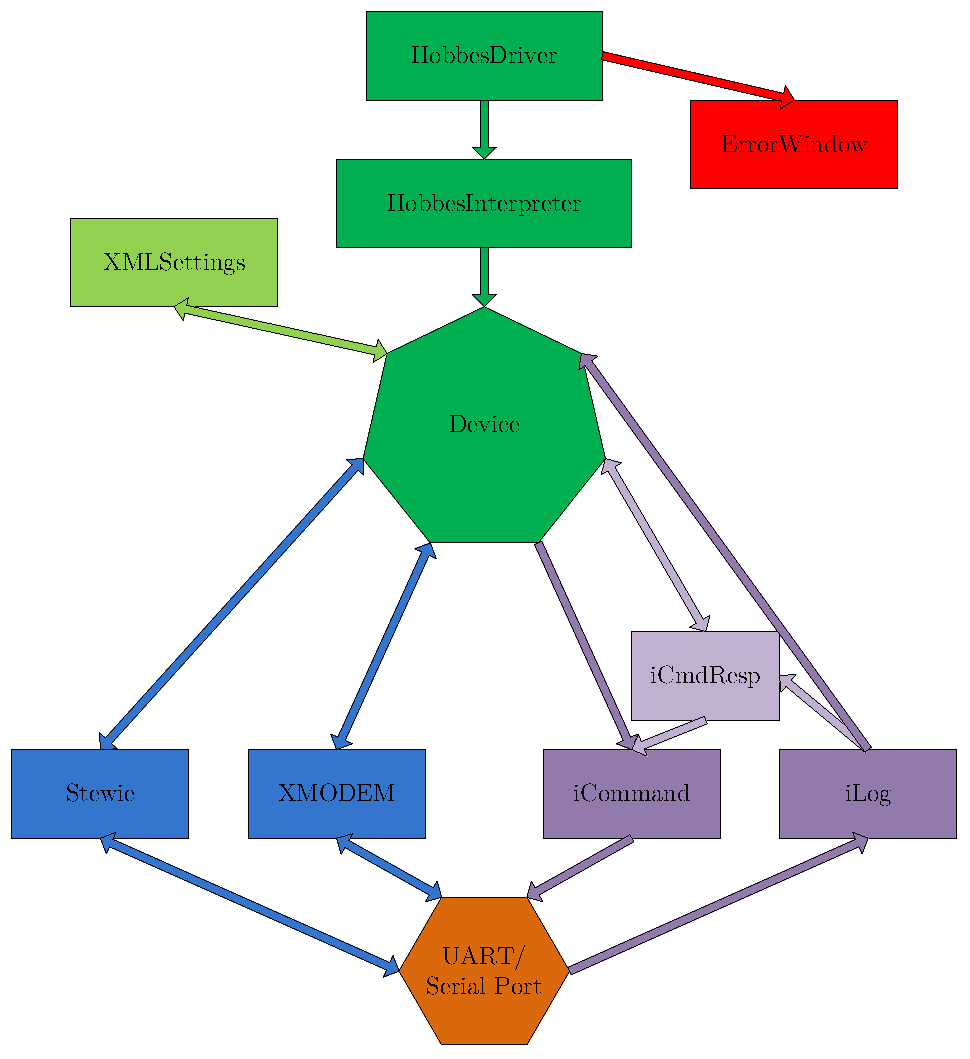
\includegraphics[scale=1]{hobbes_design.pdf}
\end{center}

\setcounter{subsection}{-1}



%
% Section 4.0
%
\subsection{HobbesDriver}
\label{4.0}

When this module is run (e.g. ``ipy.exe HobbesDriver.py''), the Hobbes program starts. This should be the only method of opening the program, for simplicity.

This module should do nothing more than start the program in a try/except block. If an exception is raised, an error window (\hyperref[4.2]{$\S4.2$}) is created and displayed.

In Hobbes 0, this module starts the program by creating an instance of the HobbesInterpreter class. Nothing is actually done with the class instance; the main loop is in the \_\_init\_\_ function of the instance.

If desired, this module can be phased out easily by moving all of the code in this module to the HobbesInterpreter module and renaming it HobbesMain or something similar.

\setcounter{subsubsection}{-1}



%
% Section 4.0.0
%
\subsubsection{Classes}
\label{4.0.0}

None.



%
% Section 4.0.1
%
\subsubsection{Functions}
\label{4.0.1}

None.



%
% Section 4.0.2
%
\subsubsection{Variables and miscellaneous}
\label{4.0.2}

None.



%
% Section 4.1
%
\subsection{HobbesInterpreter}
\label{4.1}

The program should run in a main loop here, either from this module itself or from a driver module if it exists, as Hobbes 0 does. The interpreter should do the following:

\begin{enumerate}

\item Prompt the user for input.

\item If the user enters a command that requires more input (e.g. the first line of a for loop), prompt for more input until an empty line is entered.

\item Execute the input, displaying an error if one is encountered.

\end{enumerate}

This is basically what the Python interpreter does. Hobbes 0's interpreter is slightly different; the User's Guide has more information on that.

The interpreter must be capable of doing the following:

\begin{itemize}

\item Loading (optional) scripts at startup. This should be no more than running code from a specified file. In Hobbes 0, the file is StartupScript.py in the program directory.

\item Maintaining Devices. This includes adding Devices, removing Devices, loading .icron files for Devices, and creating Python wrappers for the Devices.

\item Saving anything that can be used in a later session before exiting (normally, i.e. when the user requests an exit without any crash occuring).

\end{itemize}


\emph{Optional GUI component:} Instead of the console, there could be a window that serves as the main window of Hobbes, similar to the main window of Tigger. This window would do everything the interpreter needs to do by simply sending code to the interpreter once a certain button is clicked. This is implemented as the StartupWindow class in Hobbes 0.

\setcounter{subsubsection}{-1}



%
% Section 4.1.0
%
\subsubsection{Classes}
\label{4.1.0}

\setcounter{paragraph}{-1}



%
% Section 4.1.0.0
%
\paragraph{HobbesInterpreter}
\label{4.1.0.0}

Contains the functions that do the tasks required by the interpreter. An instance of this class is created in HobbesDriver in Hobbes 0.

This class actually is not terribly useful in Hobbes 0. The class could be removed and the functions renamed to something else if desired.



%
% Section 4.1.0.1
%
\paragraph{StartupWindow}
\label{4.1.0.1}

Provides a GUI to call the functions in HobbesInterpreter.



%
% Section 4.1.1
%
\subsubsection{Functions}
\label{4.1.1}

\setcounter{paragraph}{-1}



%
% Section 4.1.1.0
%
\paragraph{HobbesInterpreter}
\label{4.1.1.0}

Functions in the HobbesInterpreter class:

\setcounter{subparagraph}{-1}



%
% Section 4.1.1.0.0
%
\subparagraph{\_\_init\_\_()}
\label{4.1.1.0.0}

\emph{Arguments:} self - the class instance, as per Python conventions; nothing if the HobbesInterpreter class does not exist (note: I won't mention self again, since I'd otherwise have to mention it for nearly every other function)

\emph{Returns:} None (i.e. the Python equivalent of null)

Starts the Hobbes interpreter. Since this function is in a class, this is called when a HobbesInterpreter class instance is created. If this class is not implemented, the function should have a name like hobbes\_start() or something similar.

This function should do the following:

\begin{enumerate}

\item Print a startup message. Obviously, this is optional, but it would be nice to show the version number.

\item Execute startup code. This should include importing everything in the other modules so they're accessible in the interpreter, a startup script that can be edited by the user, and any other functions that may be of use. In Hobbes 0, a function of use that is imported is get\_iCommand(), described in the following section.

\item Open a startup window. This is StartupWindow in Hobbes 0. Again, this is optional, but if there is a startup window it should be started here. Also, a new thread or process must be created so the main interpreter thread doesn't lock. Hobbes 0 requires this thread to have some sort of STA state, as apparently .NET crashes otherwise.

\item Load a previous session, if it exists. Again, this is optional, and is just a convenience to the user (albeit a major convenience). The session can contain information on the serial ports Hobbes was connected to, the .icron files loaded for the Devices connected to the ports, and the location and size of the window. This session data can be saved when Hobbes exits normally.

Hobbes 0 does this with the \href{http://www.json.org/}{JSON} format, and saves the aforementioned information in Settings\textbackslash PreviousSession.hbs of the program directory with the following format:

\fontfamily{fi4}\selectfont

\begin{lstlisting}
{
    [SERIAL PORT NAME (string)]: [
        [
            [LOCATION: X COORDINATE (integer)], 
            [LOCATION: Y COORDINATE (integer)]
        ], 
        [
            [SIZE: WIDTH (integer)], 
            [SIZE: HEIGHT (integer)]
        ], 
        [PATH OF .ICRON FILE (string)]
    ]
}
\end{lstlisting}

\fontfamily{cmr}\selectfont

\item Begin an REPL (Read, Evaluate, Print Loop). A normal exit from the console would consist of the user entering ``exit'', ``hobbes.exit()'', or Control-D in the console. Note there are other possibilities, e.g. ``import os; os.\_exit(0)'' in Python, but these aren't considered ``normal'' because they don't save the session before exiting.

\item Lastly, save the session. As mentioned immediately above, only ``normal'' exits will perform this step. Saving the session consists of getting the location and size of each DeviceWindow, closing them, getting the paths of the Devices' .icron files, then writing them all to a dictionary. The dictionary is then written to Settings\textbackslash PreviousSession.hbs in the program directory (of course, this can have some other path, as long as in step 4, Hobbes is looking for the session information in the right place).

\end{enumerate}



%
% Section 4.1.1.0.1
%
\subparagraph{add\_device()}
\label{4.1.1.0.1}

\emph{Arguments:} port - the name of the serial port Hobbes should create a Device to connect to

\emph{Returns:} The Device that was created, assuming that it was created successfully

Does what you probably think it would do: add a Device. Note that Hobbes 0 implements this as addDevice(). Really, it's all up to whether you prefer identifiers with underscore\_delimiters\_with\_all\_lowercase or camelCase. This document will switch back and forth; Hobbes 0 also uses both because I switched from the latter to the former after developing most of Hobbes 0, so most of the newest additions use the former.

This function does the following:

\begin{enumerate}

\item Create a Device, using the port argument in \hyperref[4.3.1.2.0]{its constructor}

\item Check to see if the Device connected to a valid port name. If not, don't do anything with this Device and return.

\item Check to see if the port the new Device connects to is already taken up by another Device. In Hobbes 0, the port names are in the keys of the devices dictionary, so it checks by building a list comprehension and seeing if it's empty:

\fontfamily{fi4}\selectfont

\begin{lstlisting}
# check to see if there is a Device that already connects to port
# list comprehension used, of course:
# name in self.devices.keys() iterates through all port names
# if name in [port] returns True (populating the list output)
#     if there is a name match
# the leftmost name can really be anything else; as long as there is
#     something in the list, the conditional will return True
if [name for name in self.devices.keys() if name in [port]]:
    # don't mess anything up and exit the function
    print DateTime.Now.ToString('MM/dd/yy HH:mm:ss.ff ') + \
          'The device already exists!'
    return
\end{lstlisting}

\fontfamily{cmr}\selectfont

\item Set the Device's interpreter and interpreter scope correctly if needed. If the Device can access the interpreter without setting references to it, this step is unnecessary. As it is, Hobbes 0 requires this step:

\fontfamily{fi4}\selectfont

\begin{lstlisting}
# point the interpreter and interpreter scope to the correct places
device.interpreter = self.Calvin
device.interpreterScope = self.CalvinScope
\end{lstlisting}

\fontfamily{cmr}\selectfont

\item Connect the Device to the serial port. This can just consist of calling the \hyperref[4.3.1.2.1]{appropriate function} of the Device.

\item Save the port name and Device somewhere. In Hobbes 0, this means adding an entry to a dictionary whose keys, as port names, correspond to values of references to Devices.

\item Finally, return the newly-created Device. This will be useful if one wants to load a .icron file for the Device immediately after creating it.

\end{enumerate}



%
% Section 4.1.1.0.2
%
\subparagraph{remove\_device()}
\label{4.1.1.0.2}

\emph{Arguments:} port - the name of the serial port connected to the Device to be removed

\emph{Returns:} None

Again, the function name should be self-explanatory. This function removes a Device. In Hobbes 0, this is removeDevice().

This function does the following:

\begin{enumerate}

\item Try to get a reference to the Device to remove; if this fails, tell the user and exit. This would probably be something like getting a reference from the Device name repository in a try-except block, and exiting if an exception is raised.

\item If the DeviceWindow of the Device hasn't been already closed, close it. Of course, one could also attempt closing the window in a try-except block, and ignoring the exception that would be raised if the window was already closed.

\item If the serial port of the Device hasn't been already closed, close it. Basically the same thing as above with the try-except option.

\item Remove the port name and Device. In Hobbes 0, this is ``del self.devices[port]'', utilizing the Python del function. Here, there should probably be some sort of notification to the user that the Device had been removed.

\end{enumerate}



%
% Section 4.1.1.0.3
%
\subparagraph{load()}
\label{4.1.1.0.3}

\emph{Arguments:} self; dev - the Device to load the .icron file; path - the path of the .icron file

\emph{Returns:} None

Loads a .icron file from the specified path for the specified Device. If this succeeds, Hobbes goes on to create Python wrappers for the Device's iCommands and iCmdResps. Note that load() is a rather basic function name, so if one were to remove the HobbesInterpreter class she'd probably want to rename this to something more specific like load\_icron\_file().

This function firstly calls the \hyperref[4.3.1.2.5]{load\_icron\_file()} function of the Device, with the .icron file path as the argument.
If this function raises an exception for any reason, Python wrappers will not be created.

The first Python function created is one that prints to the output textbox of a DeviceWindow. It appends text to the textbox, then scrolls the text to the bottom if the user desires. This is the function in Hobbes 0:

\fontfamily{fi4}\selectfont

\begin{lstlisting}
def {0}_OUT(output):
    '''Print to the DeviceWindow's output textbox.
    Argument: output - the text to print'''
    textbox = hobbes.devices['{0}'].devWindow.OutputTextBox
    textbox.AppendText(str(output) + '\\r\\n')
    # scroll if required
    if hobbes.devices['{0}'].devWindow.scroll:
        textbox.Select(len(textbox.Text), 0)
        textbox.ScrollToCaret()
\end{lstlisting}

\fontfamily{cmr}\selectfont

Note that {0} is the port argument. This code is passed to Calvin and executed, so each Device has a unique ...\_OUT() function.

Next, Hobbes should figure out whether iCmdResp wrappers need to be created. iCmdResps are a recent addition, and are only present in GE .icron files with version number 2 and above. Reading information from icron\_header in the .icron file will be sufficient.

Hobbes now creates Python wrappers for iCommands. The following rules are followed:

\begin{itemize}

\item Each iComponent that has iCommands corresponds to a Python class.

\item Each iCommand corresponds to a Python function.

\item Each help string of an iCommand corresponds to the doc string of the Python function.

\item Each Python function does nothing more than call the send() function of an iCommand.

\item Each Python function is static, i.e. a class instance does not necessarily have to be created to call functions in the class.

\end{itemize}

And each Python function should look something like what Hobbes 0 does:

\fontfamily{fi4}\selectfont

\begin{lstlisting}
# class [dev port]_[compStr]:
#     def [cmdStr]([args]):
#         '''[documentation]'''
#         hobbes.devices[port].iCommands["[compStr]_COMPONENT"][
#             cmdIndex].send([args])
#     [cmdStr] = staticmethod([cmdStr])
\end{lstlisting}

\fontfamily{cmr}\selectfont

Depending on how iComponents and iCommands are implemented on the Device, the actual function body may vary; however, it should be clear that there is only one task to do in the function. The various [] fields are filled in using information from the Device, and iterating through each of the iComponents. The last line with ``staticmethod'' is used to make the function static.

This code isn't executed yet if we still have iCmdResp wrappers to create. They look virtually the same as iCommands, with the biggest exception being that they must return a value (again, this is directly copied from Hobbes 0):

\fontfamily{fi4}\selectfont

\begin{lstlisting}
# class [dev port]RESP_[compStr]:
#     def [cmdStr]([args]):
#         '''[documentation]'''
#         return hobbes.devices[port].iCmdResps[
#             "[compStr]_COMPONENT"][cmdIndex].respSend([args])
#     [cmdStr] = staticmethod([cmdStr])
\end{lstlisting}

\fontfamily{cmr}\selectfont

Note that the function of the iCmdResp called is respSend(), but of course this depends on how iCmdResp is implemented and it could be send() as well. Also, creation of iCmdResps should only be attempted if the .icron file supports it (GE, version >= 2).

The iCmdResp wrapper code is added onto the iCommand wrapper code (making sure there are an appropriate amount of newlines), then the whole shebang is executed by Calvin. And now you have Python wrappers! How to use them is detailed in the User's Guide, as Python help doesn't really seem to belong in a design document.



%
% Section 4.1.1.0.4
%
\subparagraph{exit()}
\label{4.1.1.0.4}

\emph{Arguments:} self

\emph{Returns:} None

Saves the session and exits Hobbes. As with other functions, this function name should be something more specific like hobbes\_exit() if there is no HobbesInterpreter class.

This function should store variable values of Devices and DeviceWindows, then write them to an external file.

The program should then close. If there is a function that exits the program immediately, it should be called. In Hobbes 0, this is ``os.\_exit(0)''. Alternatively, the function could set a boolean value that is checked periodically, and determines whether the program should continue or not.



%
% Section 4.1.1.1
%
\paragraph{StartupWindow}
\label{4.1.1.1}

Functions in the StartupWindow class:

\setcounter{subparagraph}{-1}



%
% Section 4.1.1.1.0
%
\subparagraph{\_\_init\_\_()}
\label{4.1.1.1.0}

\emph{Arguments:} self

\emph{Returns:} None

Initialize all the GUI components. There is nothing more to do.

This is a rather tedious function in Hobbes 0; it does what Designer code would do in a C\# program. If GTK+ was used in an implementation of Hobbes, Glade could be used to make the GUI initialization much simpler.



%
% Section 4.1.1.1.1
%
\subparagraph{icronFileButton\_Click()}
\label{4.1.1.1.1}

\emph{Arguments:} self; sender - the button sending the event; args - arguments from the event, which we don't need

\emph{Returns:} None

Called when icronFileButton is clicked. It should prompt the user to select a .icron file to load. Hobbes 0 uses an OpenFileDialog; GTK+ provides a GtkFileChooserDialog.



%
% Section 4.1.1.1.2
%
\subparagraph{DeviceRefreshButton\_Click()}
\label{4.1.1.1.2}

\emph{Arguments:} self; sender; args (note these are the same as above)

\emph{Returns:} None

Called when DeviceRefreshButton is clicked, and refreshes the list of serial ports Hobbes can connect to. The easiest way to accomplish this would be to get the available ports and repopulate the serial port list.



%
% Section 4.1.1.1.3
%
\subparagraph{addDeviceButton\_Click()}
\label{4.1.1.1.3}

\emph{Arguments:} self; sender; args

\emph{Returns:} None

Called when addDeviceButton is clicked (see a pattern here?). Begins a new thread that executes code generated from the text properties of the Device and .icron file components. This code should call \hyperref[4.1.1.0.1]{add\_device()} and \hyperref[4.1.1.0.3]{load()} in HobbesInterpreter.



%
% Section 4.1.1.1.4
%
\subparagraph{StartupWindow\_Closed()}
\label{4.1.1.1.4}

\emph{Arguments:} self; sender; args

\emph{Returns:} None

Called when the startup window is closed. Also executes code in a different thread; this time, the code is simply the calling of \hyperref[4.1.1.0.4]{exit()} in HobbesInterpreter. This allows the user to completely eschew the console if she wishes, as exiting does not necessarily have to be through the console.

%
% Section 4.1.1.1.5
%
\subparagraph{StopDeviceOutputButton\_Click()}
\label{4.1.1.1.5}

\emph{Arguments:} self; sender; args

\emph{Returns:} None

Called when StopDeviceOutputButton is clicked. Gets device argument from DeviceComboBox, this method begins a new thread that suspends output and dumps to a file the logCache of an existing device window.


%
% Section 4.1.1.1.6
%
\subparagraph{execute\_code()}
\label{4.1.1.1.6}

\emph{Arguments:} self

\emph{Returns:} None

Executes code by passing it to the interpreter. This should always execute in a different thread to prevent locking anything up. If an exception is raised, it is shown as a popup. Note there should be an appropriate facility to pass the code to execute into the thread as a parameter. In IronPython one can use ParameterizedThreadStart (.NET) or the threading module (CPython).



%
% Section 4.1.1.1.7
%
\subparagraph{run()}
\label{4.1.1.1.7}

\emph{Arguments:} self

\emph{Returns:} None

Runs the StartupWindow. In Hobbes 0 this is just ``Application.Run(self)'' in a try-except block, where any exception opens an ErrorWindow class instance.



%
% Section 4.1.2
%
\subsubsection{Variables and miscellaneous}
\label{4.1.2}

Hobbes 0 adds the contrib/ folder to the path and adds the IronPython.dll file to the CLR at the module level.

At the module level, there are a couple variables:

\setcounter{paragraph}{-1}



%
% Section 4.1.2.0
%
\paragraph{hobbes\_version}
\label{4.1.2.0}

A string containing the version of Hobbes, e.g. ``0.4-rc15''. This shows up in the console during startup and the startup window in Hobbes 0.



%
% Section 4.1.2.1
%
\paragraph{program\_path}
\label{4.1.2.1}

A string containing the file path of the program.

\emph{This variable should be unnecessary.} Usually something like os.getcwd() (in Python) would work. However, .NET has a \sout{bug} feature where opening an OpenFileDialog or SaveFileDialog changes the current directory. Which is fine if we never need the actual path of the program...but we do for things like running an untarring program in the directory. Thus, we use some Python hackery to get the full path of the HobbesInterpreter.py file, which happens to be the program directory, and save it in a variable for convenience.



%
% Section 4.1.2.2
%
\paragraph{HobbesInterpreter}
\label{4.1.2.2}

Variables in the HobbesInterpreter class:

\setcounter{subparagraph}{-1}



%
% Section 4.1.2.2.0
%
\subparagraph{devices}
\label{4.1.2.2.0}

One of the more important variables in the program. Contains information on every Device that's currently connected to a serial port (which normally should be all of them). In Hobbes 0, this is implemented as a Python dictionary, where the keys are serial port names and the values are references to Devices connected to said port names. For example, if there is one Device currently in existence connected to serial port COM42, the devices variable in Hobbes 0 would look like ``\{`COM42': $<$Device.Device instance at 0xSOME\_MEMORY\_LOCATION$>$\}''. Every Device can be accessed through this variable.



%
% Section 4.1.2.2.1
%
\subparagraph{Calvin}
\label{4.1.2.2.1}

The actual interpreter. It could interpret any suitable scripting language, but in Hobbes 0 it interprets Python, and scripting in Python seems to be the one of the easiest options, so I would recommend it's a Python interpreter. Of course, this should have a function for executing code passed in to it.



%
% Section 4.1.2.2.2
%
\subparagraph{CalvinScope}
\label{4.1.2.2.2}

The scope of Calvin. Includes all the variables that are set in Calvin. This may or may not be necessary, depending on the implementation of Hobbes; in Hobbes 0, this is mandatory for executing code, as a function in Calvin is used to merely compile the code--it is actually executed in a function under CalvinScope.



%
% Section 4.1.2.2.3
%
\subparagraph{startupWindow}
\label{4.1.2.2.3}

A simple variable containing a reference to a StartupWindow class instance.



%
% Section 4.1.2.3
%
\paragraph{StartupWindow}
\label{4.1.2.3}

There are \emph{a lot} of variables here that are all related to the GUI. I won't be specific as to how the GUI should be implemented in terms of what variables there should be, and how it should look, as the objectives of the GUI outlined above should be sufficient. If you're actually very interested in what all the variables are, check out the \_\_init\_\_() function of the StartupWindow class in Hobbes 0.



%
% Section 4.2
%
\subsection{ErrorWindow}
\label{4.2}

If you're lucky, this module will never be used. But crashes happen, so the ErrorWindow class in this module will be used occasionally.

Note that the class actually isn't necessary. Instead of creating an ErrorWindow class instance when an exception is raised, one could simply ``import ErrorWindow'' and modify the code such that everything gets called at the module level. Hobbes 0 uses a class though.

\setcounter{subsubsection}{-1}



%
% Section 4.2.0
%
\subsubsection{Classes}
\label{4.2.0}

\setcounter{paragraph}{-1}



%
% Section 4.2.0.0
%
\paragraph{ErrorWindow}
\label{4.2.0.0}

Contains a window that is shown when something bad happens. In Hobbes 0, this doesn't necessarily mean the entire program's crashed. If a DeviceWindow encounters an error, the thread running it will exit, while the main thread will soldier on.

Also writes the exception information/stack trace to an error log. This is ErrorLog.txt in the program directory in Hobbes 0.



%
% Section 4.2.1
%
\subsubsection{Functions}
\label{4.2.1}

\setcounter{paragraph}{-1}



%
% Section 4.2.1.0
%
\paragraph{ErrorWindow}
\label{4.2.1.0}

Functions in the ErrorWindow class:

\setcounter{subparagraph}{-1}



%
% Section 4.2.1.0.0
%
\subparagraph{\_\_init\_\_()}
\label{4.2.1.0.0}

Creates all the GUI components, then displays the window. This freezes the thread that the error occurred on.

The only real mandatory GUI component is a button to close the error window.



%
% Section 4.2.1.0.1
%
\subparagraph{closeButton\_Click()}
\label{4.2.1.0.1}

Called when the close button is clicked, and closes the window (if it wasn't already obvious enough).



%
% Section 4.2.2
%
\subsubsection{Variables and miscellaneous}
\label{4.2.2}

The variable \hyperref[4.1.2.1]{program\_path} is not available here, so Hobbes 0 just repeats the Python stuff to create it here. Hobbes 0 does this to add an icon to the error window:

\fontfamily{fi4}\selectfont

\begin{lstlisting}
self.Icon = Icon(os.path.dirname(os.path.realpath(__file__)) +
            "\\hobbesicon.ico")
\end{lstlisting}

\fontfamily{cmr}\selectfont

\setcounter{paragraph}{-1}



%
% Section 4.2.2.0
%
\paragraph{ErrorWindow}
\label{4.2.2.0}

Again, peruse Hobbes 0 code if you are interested in the detailed design of the GUI. If you do implement it a completely different way...at least keep the comic. Or put in another Calvin and Hobbes one. But I thought the one that's there seemed to fit the moment.



%
% Section 4.3
%
\subsection{Device}
\label{4.3}

All communication with the serial port should involve this module. Although sending of bytes to the serial port is handled by the iCommand module and parsing of bytes received from the port is handled by the iLog module, the iCommands and iLogs contained in a .icron file are stored in a Device class instance.

There should also be an additional class that contains a separate window, which at the minimum allows iLog output to be printed to it. Technically, this is optional, but having all iLog output go to the console would quickly get very annoying.

\setcounter{subsubsection}{-1}



%
% Section 4.3.0
%
\subsubsection{Classes}
\label{4.3.0}

\setcounter{paragraph}{-1}



%
% Section 4.3.0.0
%
\paragraph{Device}
\label{4.3.0.0}

Connects to a serial port. Contains iCommands and iLogs to send/parse bytes to/from the serial port. Also parses bytes when bootloading/flashing through the port by Stewie or XMODEM.



%
% Section 4.3.0.1
%
\paragraph{DeviceWindow}
\label{4.3.0.1}

Contains a textbox where iLog output is printed. Additionally provides another textbox for code input to Calvin, and optionally methods for opening other GUI components. There should also be options for controlling the display of the text in the output textbox in the window (e.g. clearing all the text).



%
% Section 4.3.1
%
\subsubsection{Functions}
\label{4.3.1}

In addition to the functions in the Device and DeviceWindow classes, there are some additional module-level functions. These are optional, but may be very useful depending on the type of user.

\setcounter{paragraph}{-1}



%
% Section 4.3.1.0
%
\paragraph{crc16()}
\label{4.3.1.0}

\emph{Arguments:} data - an 8-bit integer to calculate the CRC-16 on; last - the starting CRC-16 to use (i.e. the last one calculated)

\emph{Returns:} The new CRC-16 calculated on the data input

Surprisingly enough, calculates the CRC-16 of an 8-bit input using a previous CRC-16.

The calculation of the CRC-16 is done as follows:

\begin{enumerate}

\item Take the bitwise NOT of the last CRC-16, and if necessary, mask it with 0xFFFF to ensure the final result is 16 bits. Store this result in a variable; in Hobbes 0 this variable is called ``next'', and will henceforth be referred to as such.

\item Check to see if the value of the least significant bit in the 8-bit input matches the value of the least significant bit in ``next''. If so, shift the bits of ``next'' to the right by one. If they don't match, do the aforementioned right bitwise shift by one, but also XOR ``next'' by 0xA001.

\item Do the same check on the remaining seven bits, from least significant to most significant. That is, after the first check, check the second least significant bit, then the third last significant bit, and so on.

\item Take the bitwise NOT of ``next'', and mask with 0xFFFF if necessary. This is the final CRC-16. Return this value.

\end{enumerate}

Note that if the data input is, say, 64 bits, the CRC-16 will likely be incorrect. If the data to calculate the CRC-16 on is greater than 8 bits, it should not be too difficult to create a loop where the CRC-16 is calculated on each 8-bit segment of the data.

In case the CRC-16 calculation procedure above was too confusing, here's Hobbes 0's implementation (which is probably even more confusing):

\fontfamily{fi4}\selectfont

\begin{lstlisting}
# the only peculiar thing is masking with 0xFFFF; this limits Python's ~
#     operator to 16 bits
next = ~last & 0xFFFF
for i in range(8):
    if ((data >> i) & 1 == next & 1):
        next >>= 1
    else:
        next >>= 1
        next ^= 0xA001
    
return ~next & 0xFFFF
\end{lstlisting}

\fontfamily{cmr}\selectfont



%
% Section 4.3.1.1
%
\paragraph{availablePorts()}
\label{4.3.1.1}

\emph{Arguments:} None. (That is, there are no arguments. Not the Python keyword None.)

\emph{Returns:} A collection of the available serial ports on the host system.

This function can be implemented in many different ways. It's not even used in Hobbes 0 as it were, since .NET provides SerialPort.GetPortNames(). However, in an alternate implementation of Hobbes, .NET won't be available, so there needs to be a way of finding all the serial ports that are connected.

One way of implementing this function is checking the OS, i.e. the value of sys.platform (assuming the Hobbes implementation is in Python) and enumerating a list of serial ports depending on the OS:

\begin{itemize}

\item In Windows, sys.platform would return ``win32'' or ``cli'', depending on the implementation (in IronPython it would be the latter), and the \_winreg module (assuming Python 2 is used; it's winreg in Python 3) would be used to read from the Windows registry. In Hobbes 0:

\fontfamily{fi4}\selectfont

\begin{lstlisting}
ports = []
# we can only read from the Windows registry if (surprise) we're on Windows
if sys.platform == "win32" or sys.platform == "cli":
    # get access to the serial port registry entry
    key = winreg.OpenKey(winreg.HKEY_LOCAL_MACHINE,
                            r"HARDWARE\DEVICEMAP\SERIALCOMM")
    # find the number of values in the entry, which corresponds to the
    #     number of serial ports connected to the system
    for i in range(winreg.QueryInfoKey(key)[1]):
        # append each port name to the ports list
        ports.append(str(winreg.EnumValue(key, i)[1]))
        
    # close the handler
    key.Close()
\end{lstlisting}

\fontfamily{cmr}\selectfont

Note that ``import \_winreg as winreg'' is performed at the module level in Hobbes 0 to avoid the annoying underscore.

\item In Linux, sys.platform would return ``linux2'', and all serial ports would show up in /dev/ttyS*. Searching there would be sufficient.

\item In OS X, sys.platform would return ``darwin''...refer to what Hobbes 0 does. (Obfuscation is fun. I didn't want to make it \emph{too} obvious what I was doing there.)

\end{itemize}

Lastly, return the collection of ports. Sorting the collection, if necessary, would be optional but perhaps more convenient to the user. In Python this would just be ``return sorted(ports)''.



%
% Section 4.3.1.2
%
\paragraph{Device}
\label{4.3.1.2}

Functions in the Device class:

\setcounter{subparagraph}{-1}



%
% Section 4.3.1.2.0
%
\subparagraph{\_\_init\_\_()}
\label{4.3.1.2.0}

\emph{Arguments:} self; programPath - the path of Hobbes program (see \hyperref[4.1.2.1]{program\_path}); port - the name of the serial port to connect to; settings - the path of the XMLSettings file to load for Device settings

\emph{Returns:} None

This function should do, at minimum, the following:

\begin{itemize}

\item Initialize any variables that need initializing, including any lists, dictionaries, class instances, etc. Hobbes 0 also includes all the variables that are used in the class instance here regardless of whether they need to be initialized, simply to have a convenient list of all the variables used (since it's Python, variables don't need to be declared if they have something immediately assigned to them).

\item Set the port name of the serial port assuming it is valid, i.e. if it is in the list of available ports. If it isn't, be helpful and print a list of the available serial ports.

\item Load Device settings. This uses the settings argument, which defaults to a blank string. If this default is used, default Device settings should be loaded. The default settings should be in an external file; it's in Settings\textbackslash DefaultDeviceSettings.xml in Hobbes 0.

\end{itemize}



%
% Section 4.3.1.2.1
%
\subparagraph{connect()}
\label{4.3.1.2.1}

\emph{Arguments:} self

\emph{Returns:} None

Opens the serial port of the Device class instance, or reopens it if it's already open. Load the settings for the serial port: the baud rate, parity, data bits, stop bits, handshake, write timeout, and read timeout.

Following this, create a DeviceWindow class instance and open it in a new thread. There should also be some notification that tells the user the Device has connected properly with the given settings.

\emph{The Device settings should be deprecated.} It's not necessary, and was only included in Hobbes 0 as Tigger legacy. The only parameters that need to be specifically set are the serial port name, and possibly the baud rate if 115200 isn't the default.



%
% Section 4.3.1.2.2
%
\subparagraph{DataReceivedHandler()}
\label{4.3.1.2.2}

\emph{Arguments:} self; sender - the serial port calling this function; args

\emph{Returns:} None

Called when bytes are received from the serial port of the Device class instance.

In .NET, this handler is called once when data is received, not every time a byte is received. For the most part, this seems to work fine. In a non-.NET implementation of Hobbes, there could be a separate thread that runs and parses bytes if it is determined that there are bytes to read from the serial port, and sleeps if there is nothing to read. This might look something like this, with \href{http://pyserial.sourceforge.net/}{PySerial} and the Python threading and time modules:

\fontfamily{fi4}\selectfont

\begin{lstlisting}
import serial, threading, time

ser=serial.Serial([SERIAL PORT], 115200)

def read_thread():
    while True:
        try:
            if ser.inWaiting():
                [do stuff]
            else:
                time.sleep(0.01)
        except AttributeError:
        # raised when we try to read from a closed port
        # may occur during exit
            pass

thread=threading.Thread(target=read_thread)
thread.daemon = True # ensure the program can actually exit
thread.start()
\end{lstlisting}

\fontfamily{cmr}\selectfont

This function should first read a byte from the serial port. One could read more, but everything parsing received bytes would have to iterate through the block of received bytes and it would generally be rather messy.

Next, something should be done with the byte, depending on what's happening:

\begin{itemize}

\item If we're currently processing an iLog, or the byte is greater than or equal to 240, parse the byte using the iLog module. The latter case means that the byte is a header for an iLog.

\item Otherwise, if the byte matches a byte we're waiting for during flash, and it's not equal to 0, set an event that notifies another function that the appropriate byte has been received. Note the non-zero check; in Hobbes 0, the waiting flash byte is 0 when it's not being used. (It just occurred to me that it could be -1, which would be simpler, but you never know what could happen.)

\item Otherwise, if the byte is 21, it's an ASCII NAK. In this case, further assess the situation. If we're waiting for a flash byte, we're flashing, and as a NAK was received, we need to resend the packet. This could involve setting the event that is mentioned in the second item above, while also setting a variable that is only True when a NAK is received to True. In Hobbes 0, there is a variable of the sort named ``self.flashNAK''. If we're not waiting for anything, then output the timestamp and NAK message to a DeviceWindow.

\item Otherwise, if the byte received is part of a bootload message when flashing using Stewie, increment a counter that iterates across the length of set lists containing the bytes of each message. In other words, check if the entire bootload message has been received. If it has, print it.

\item Finally, if none of the above conditions were satisfied, print a message saying an unknown byte was received.

\end{itemize}

Note that this entire segment of code should be wrapped in a try-except block. A SystemError (in Hobbes 0) could occur if Hobbes attempts to read from a closed serial port, which could happen if the program is closing and the port is automatically closed. If any other error is encountered, appropriate ErrorWindow handling should occur.



%
% Section 4.3.1.2.3
%
\subparagraph{\_\_parseNAK()}
\label{4.3.1.2.3}

\emph{Arguments:} self

\emph{Returns:} None

\emph{Optional function.} This can handle the case where the byte read from the serial port is a NAK, and an iLog isn't being processed. The rationale for this function would be making the \hyperref[4.3.1.2.2]{DataReceivedHandler()} function a little shorter and probably a bit easier to read.

Also, it of course doesn't have to be a Python ``private'' function; ``parse\_NAK()'' would be fine too.



%
% Section 4.3.1.2.4
%
\subparagraph{icron\_untar()}
\label{4.3.1.2.4}

\emph{Arguments:} self; name - the name of the .icron file to extract data from

\emph{Returns:} the data extracted, as a string

Untars a file from a .icron file. The .icron file is in fact a .tar.bz2 file, so in CPython the \href{http://docs.python.org/library/tarfile.html}{tarfile} module could be used to read the .icron file. In Hobbes 0, however, bz2 is not supported in IronPython, so an external program must be used to extract files from the .icron file. This is exactly what Tigger does.

The function needs to extract the specific file from the .icron file, and write the standard output to a string. Once this is done, the standard error stream should be checked to ensure it's empty, and the standard output is not empty. If one or both of these conditions are not met, something went wrong and an exception should be raised. In the case that everything is fine and dandy, return the string that standard output was written to.

This is actually quite tedious in Tigger and Hobbes 0; the .NET Process and ProcessStartInfo classes are used, and many inane variables must be set to extract a file correctly. As noted, CPython's tarfile module would be quite a bit easier to use and understand.



%
% Section 4.3.1.2.5
%
\subparagraph{load\_icron\_file()}
\label{4.3.1.2.5}

\emph{Arguments:} self; path - the path of the .icron file to load

\emph{Returns:} None

Untars a .icron file to read the icomponent, icmd, ilog, and possibly icmdresp files into corresponding data structures of the Device.

Firstly, there should be a check to ensure the path points to a file, and bsdtar.exe in the program directory exists. If one of these don't exist, an exception should be raised.

The path argument should be saved in an instance variable, as it will be used later.

Next, the ``icron\_header'' file is extracted from the .icron file. The \hyperref[4.3.1.2.4]{icron\_untar()} function is used here, if it was implemented. This file contains an assortment of keys and values, which must be stored somewhere. In Hobbes 0, they are stored in an XMLSettings class instance.

Now, the list of iComponents is retrieved by untarring the file listed under the key ``icomponent'' in icron\_header. This file is formatted as follows:

\fontfamily{fi4}\selectfont

\begin{lstlisting}
components:
C:[NAME]_COMPONENT
C:[NAME]_COMPONENT
C:[NAME]_COMPONENT
[...]
\end{lstlisting}

\fontfamily{cmr}\selectfont

For each line, the ``C:'' is removed and the remaining string is stored in a list.

Next, iCommands are retrieved by untarring the file listed under the key ``icmd'' in icron\_header. This file is formatted as follows:

\fontfamily{fi4}\selectfont

\begin{lstlisting}
component:[NAME]_COMPONENT
F:[function] H:"[help string]" A:[argument(s); void if there are no arguments]
F:[function] H:"[help string]" A:[argument(s); void if there are no arguments]
[...]
component:[NAME]_COMPONENT
F:[function] H:"[help string]" A:[argument(s); void if there are no arguments]
F:[function] H:"[help string]" A:[argument(s); void if there are no arguments]
[...]
\end{lstlisting}

\fontfamily{cmr}\selectfont

These iCommands are stored in a dictionary. Hobbes reads this file line by line. If the line begins with ``component'', Hobbes creates a new dictionary entry, with the component name as the key. The values are then added as iCommand class instances. Note that the parsing of the line is done in the iCommand \hyperref[4.5.1.0.0]{\_\_init\_\_()} function.

Next, iLogs are retrieved by untarring the file listed under the key ``ilog'' in icron\_header. This file is formatted as follows, for LG1 .icron files that are version 4 or later and GE .icron files that are version 2 or later:

\fontfamily{fi4}\selectfont

\begin{lstlisting}
component:[NAME]_COMPONENT
L:[ILOG NAME] S:[iLog string]
L:[ILOG NAME] S:[iLog string]
[...]
component:[NAME]_COMPONENT
L:[ILOG NAME] S:[iLog string]
L:[ILOG NAME] S:[iLog string]
[...]
\end{lstlisting}

\fontfamily{cmr}\selectfont

And for older .icron files:

\fontfamily{fi4}\selectfont

\begin{lstlisting}
component:[NAME]_COMPONENT
S:[iLog string]
S:[iLog string]
[...]
component:[NAME]_COMPONENT
S:[iLog string]
S:[iLog string]
[...]
\end{lstlisting}

\fontfamily{cmr}\selectfont

Note that older .icron files do not contain an iLog name identifier. These were added in recent .icron files to identify iLogs more easily, which in turn makes iCmdResps easier to implement.

The iLogs are stored in a dictionary, similar to how iCommands are stored. Again, parsing is done in an \hyperref[4.6.1.4.0]{\_\_init\_\_()} function, and there should be an extra parameter specifying if ``L:[ILOG NAME]'' needs to be parsed or not.

Next, iCmdResps are retrieved by untarring the file listed under the key ``icmdresp'' in icron\_header. First though, there should be a check to see if the .icron file is GE and version 2 or above, as icmdresp files only exist in those .icron files. Even if it is GE version 2+, there may not be an icmdresp file, so untarring should be done in a try-except block where any exception raised can be safely ignored. The file is formatted as follows:

\fontfamily{fi4}\selectfont

\begin{lstlisting}
C:[NAME]_COMPONENT
R:[response name] C:[iCommand name] L:[iLog name] A:[argument of iLog to return]
\end{lstlisting}

\fontfamily{cmr}\selectfont

If there is an icmdresp file, and it is extracted to a string successfully, it is stored in an iCmdResps dictionary.

Untarring/extraction is now complete. There is one more very important thing to do, and that is setting up a handler to parse received bytes. In Hobbes 0 this is simple: a function is attached to the SerialPort's DataReceived handler.

\fontfamily{fi4}\selectfont

\begin{lstlisting}
# and *now* start parsing received bytes
# this avoids weird stuff happening when an .icron file hasn't been
#     loaded yet, but a bunch of bytes have been received and parsed
# set a function that will be called when data is received from the
#     serial port
self.serialPort.DataReceived += self.DataReceivedHandler
\end{lstlisting}

\fontfamily{cmr}\selectfont

In CPython, .NET is not available, so the convenient (albeit possibly unreliable) event is not available. Thus, a thread running an infinite loop checking if bytes are in the serial port's buffer could be created and started; see \hyperref[4.3.1.2.2]{DataReceivedHandler()} for example code.

\emph{Optional GUI components:} If there is a DeviceWindow, the title of it should be changed to include the file path of the new .icron file. If desired, the directory containing the .icron file could be watched for deletions, and a function set up to be called if deleting occur. This function is \hyperref[4.3.1.2.6]{icronFileChanged()} in Hobbes 0. And if there is a ``Reload .icron File'' button in the DeviceWindow, ensure its font colour is black.



%
% Section 4.3.1.2.6
%
\subparagraph{icronFileChanged()}
\label{4.3.1.2.6}

\emph{Arguments:} self; sender; args

\emph{Returns:} None

A simple function that serves as a notification to the user that the .icron file may have to be reloaded (if she's paying attention). This could be anything from changing a colour somewhere to popping up an animation of a screaming face. As it is, Hobbes 0 does the relatively tame notification of changing the font colour of the ``Reload .icron File'' button from black to red.



%
% Section 4.3.1.2.7
%
\subparagraph{printToDeviceWindow()}
\label{4.3.1.2.7}

\emph{Arguments:} self; output - the text string to be printed in the DeviceWindow

\emph{Returns:} None

Takes a string as input to be displayed in the DeviceWindow.  First checks to see if ouput has been suspended, if not the messages will begin printing.  Also checks to see whether or not auto scroll is enabled.

%
% Section 4.3.1.2.8
%
\subparagraph{update\_text()}
\label{4.3.1.2.8}

\emph{Arguments:} self; newText - the text string to update the window title to.

\emph{Returns:} None

Takes a string as input to be displayed as the title of the window.  Called when programming a device and invoked onto GUI thread.


%
% Section 4.3.1.3
%
\paragraph{DeviceWindow}
\label{4.3.1.3}

Functions in the DeviceWindow class follow. Note most of these are handlers for button clicking events; as a result, if some buttons aren't implemented, there isn't any need for the functions connected to them.

\setcounter{subparagraph}{-1}



%
% Section 4.3.1.3.0
%
\subparagraph{\_\_init\_\_()}
\label{4.3.1.3.0}

\emph{Arguments:} self; dev - the Device to create a DeviceWindow for

\emph{Returns:} None

As with all GUI initialization functions, there is not a lot to specify here. The dev argument is used to save a reference to the Device for future use, and there are a couple of default values set: auto scrolling occurs and iLog suspension does not occur by default.

There is a little bit of code that isn't extremely tedious though; it creates a context menu (the pop-up menu when one right clicks in a textbox) and connects it to the input and output textboxes in Hobbes 0. However, this is only necessary for .NET because, well, it's .NET; GTK+ does context menus fine.



%
% Section 4.3.1.3.1
%
\subparagraph{suspchk\_CheckedChanged()}
\label{4.3.1.3.1}

\emph{Arguments:} self; sender; args

\emph{Returns:} None

Called when the ``Suspend iLogs'' checkbox is clicked. Modifies whether iLogs are suspended or not. Also, if the ``Suspend iLogs'' checkbox becomes unchecked, the \hyperref[4.3.2.2.23]{log cache} is printed.



%
% Section 4.3.1.3.2
%
\subparagraph{autochk\_CheckedChanged()}
\label{4.3.1.3.2}

\emph{Arguments:} self; sender; args

\emph{Returns:} None

Called when the ``Auto Scroll'' checkbox is clicked. Modifies whether the output textbox scrolls automatically or not.



%
% Section 4.3.1.3.3
%
\subparagraph{SendButton\_Click()}
\label{4.3.1.3.3}

\emph{Arguments:} self; sender; args

\emph{Returns:} None

Called when the ``Send'' button is clicked. Executes, then clears, the code in the input textbox. If desired, the executed code can be printed to the output textbox with Python prompts (``$>>>$'', ``...''). If auto scroll exists and is enabled, the output textbox should scroll. Finally, a new thread is started to execute the code.



%
% Section 4.3.1.3.4
%
\subparagraph{ClearInputButton\_Click()}
\label{4.3.1.3.4}

\emph{Arguments:} self; sender; args

\emph{Returns:} None

Called when the ``Clear'' button (located under the input textbox) is clicked. Clears the input textbox of all text.

Side note: this is a good example of a GUI component doing a task that could alternatively be accomplished by entering something in the console; in this case something like ``hobbes.devices[`COM42'].InputTextBox.Clear()''.



%
% Section 4.3.1.3.5
%
\subparagraph{SaveButton\_Click()}
\label{4.3.1.3.5}

\emph{Arguments:} self; sender; args

\emph{Returns:} None

Called when the ``Save...'' button is clicked. Prompts the user for a location to save the text in the input textbox. In Hobbes 0, a SaveFileDialog is used. Once the path is selected, all of the text in the input textbox is written to the file at the path.



%
% Section 4.3.1.3.6
%
\subparagraph{LoadButton\_Click()}
\label{4.3.1.3.6}

\emph{Arguments:} self; sender; args

\emph{Returns:} None

Called when the ``Load...'' button is clicked. Prompts the user for a file to load into the input textbox. Hobbes 0 uses an OpenFile Dialog. Once the path is selected, the text of the input textbox is entirely replaced with everything read from the file.

Note that Unix newlines (LFs) don't play nicely with Windows textboxes, which use Windows newlines (CR LFs). As a result, in Hobbes 0, there is an extra couple of commands performed on the text read from the file. First, any Windows newlines are converted to Unix newlines by replacing all occurrences of ``\textbackslash r\textbackslash n'' with ``\textbackslash n''. Then, the reverse is done; that is, all Unix newlines are then converted to Windows newlines. Note that Unix newlines in the file are thus converted to Windows newlines, while existing Windows newlines are kept as such. And of course, no one cares about silly Macs and their CR newlines.



%
% Section 4.3.1.3.7
%
\subparagraph{iCommandsButton\_Click()}
\label{4.3.1.3.7}

\emph{Arguments:} self; sender; args

\emph{Returns:} None

Called when the ``iCommands'' button is clicked. Shows an iCommandWindow.



%
% Section 4.3.1.3.8
%
\subparagraph{ReconnectButton\_Click()}
\label{4.3.1.3.8}

\emph{Arguments:} self; sender; args

\emph{Returns:} None

Called when the ``Reconnect'' button is clicked. First, this function makes sure that the serial port of the Device is in the list of available ports; if not, it loops, so it is entirely possible that a thread freezes here as it is. If there is a match (and there should be), the Device reconnects to the serial port. This has actually been useful on occasion when bytes are inexplicably not being read from the serial port.



%
% Section 4.3.1.3.9
%
\subparagraph{ClearOutputButton\_Click()}
\label{4.3.1.3.9}

\emph{Arguments:} self; sender; args

\emph{Returns:} None

Called when the ``Clear Output'' button is clicked. Clears the output textbox.



%
% Section 4.3.1.3.10
%
\subparagraph{iLogsButton\_Click()}
\label{4.3.1.3.10}

\emph{Arguments:} self; sender; args

\emph{Returns:} None

Called when the ``iLogs'' button is clicked. Shows an iLogWindow.



%
% Section 4.3.1.3.11
%
\subparagraph{ReloadIcronButton\_Click()}
\label{4.3.1.3.11}

\emph{Arguments:} self; sender; args

\emph{Returns:} None

Called when the ``Reload .icron File'' button is clicked. Reloads the .icron file of the Device by repopulating the iComponents, iCommands, etc. data collections. In Hobbes 0, this function creates code to use \hyperref[4.1.1.0.3]{load()} on the appropriate Device, and executes the code in a new thread.

The user should call this function whenever a change is made in firmware. If there is any change to the iComponents, iCommands, etc., there will be an obvious incompatibility between the .icron file loaded in the Device and the .icron file containing the firmware that had been flashed to the board. This is why Hobbes 0 watches the directory containing the .icron file for deletions, and changes the colour of ``Reload .icron File'' if there is a deletion.



%
% Section 4.3.1.3.12
%
\subparagraph{BootloadButton\_Click()}
\label{4.3.1.3.12}

\emph{Arguments:} self; sender; args

\emph{Returns:} None

Called when the ``Bootload'' button is clicked. Bootloads the board in a new thread.

The Stewie protocol is used if the ``project'' key in the .icron file starts with ``lg1'', signifying that the .icron file is for LG1 firmware or an LG1 test harness. Otherwise, the .icron file is for GE (note Hobbes won't support anything other than LG1 or GE as it is) and the XMODEM protocol is used.



%
% Section 4.3.1.3.13
%
\subparagraph{FlashButton\_Click()}
\label{4.3.1.3.13}

\emph{Arguments:} self; sender; args

\emph{Returns:} None

Called with the ``Flash'' button is clicked. Flashes the board in a new thread.

This function is somewhat similar to \hyperref[4.3.1.3.12]{BootloadButton\_Click()}. However, an iCommand is sent first. This iCommand is the first one in ``TOPLEVEL\_COMPONENT'', which should be ``xmodem\_new\_image''. If not, flashing should not go ahead. If it is, it should be sent, which results in the board beginning to send NAKs. A new thread is then started to flash the board using the XMODEM protocol.



%
% Section 4.3.1.3.14
%
\subparagraph{XMODEMSend()}
\label{4.3.1.3.14}

\emph{Arguments:} self

\emph{Returns:} None

Whatever happens here, the function sendFileByXMODEM() is called at least once. Everything sent to the board in \hyperref[4.9.1.0]{the function} uses XMODEM.

\begin{itemize}

\item If the .icron file is for a test harness, the ``test\_image'' file in the .icron file is sent.

\item If the .icron file is for GE, the ``flash\_writer'' file is sent, followed by ``main\_firmware''.

\item If the .icron file is for LG1, the ``flash\_writer2'' file is sent, followed by ``main\_firmware''.

\end{itemize}



%
% Section 4.3.1.3.15
%
\subparagraph{StewieSend()}
\label{4.3.1.3.15}

\emph{Arguments:} self

\emph{Returns:} None

Whatever happens here, the function \hyperref[4.8.1.0]{sendFileByStewie()} is called at least once.

If the .icron file is for a test harness, the ``test\_image'' file is sent by Stewie.

Otherwise, if the .icron file is for LG1, the ``flash\_writer'' file is sent by Stewie, followed by ``main\_firmware'' sent by XMODEM.



%
% Section 4.3.1.3.16
%
\subparagraph{DeviceWindow\_Closed()}
\label{4.3.1.3.16}

\emph{Arguments:} self; sender; args

\emph{Returns:} None

Called when the DeviceWindow is closed. Executes code that calls \hyperref[4.1.1.0.2]{remove\_device()} to remove the Device containing the DeviceWindow being closed (note in Hobbes 0, removeDevice() is called instead). The execution of the code should be in a new thread.



%
% Section 4.3.1.3.17
%
\subparagraph{execute\_code()}
\label{4.3.1.3.17}

\emph{Arguments:} self; code - the code to execute

\emph{Returns:} None

Very similar to the \hyperref[4.1.1.1.5]{execute\_code()} function in the StartupWindow class, but here the \hyperref[4.3.2.2.6]{interpreter} and \hyperref[4.3.2.2.7]{interpreterScope} variables are used for code execution.

In addition, the input textbox is cleared regardless of whether the code executes without any problems or not. If this function was called from \hyperref[4.3.1.3.3]{SendButton\_Click()}, the desired effect is achieved. If this function was called from \hyperref[4.3.1.3.16]{DeviceWindow\_Closed()}, nothing happens. But nothing bad happens either.



%
% Section 4.3.1.3.18
%
\subparagraph{run()}
\label{4.3.1.3.18}

\emph{Arguments:} self

\emph{Returns:} None

Runs the DeviceWindow. In Hobbes 0 this is just ``Application.Run(self)'' in a try-except block, where any exception opens an ErrorWindow class instance.



%
% Section 4.3.1.3.19
%
\subparagraph{aliasButton\_Clicked()}
\label{4.3.1.3.19}

\emph{Arguments:} self; sender; args

\emph{Returns:} None

Called when one of the nine alias buttons is clicked in either the iCommand window or Device window. Executes the code saved in that alias button in a new thread.

%
% Section 4.3.1.3.20
%
\subparagraph{dev\_dumpLogCache()}
\label{4.3.1.3.20}

\emph{Arguments:} self

\emph{Returns:} None

Calls the dumpLogCache method in the iLog module with the device as the argument.


%
% Section 4.3.2
%
\subsubsection{Variables and miscellaneous}
\label{4.3.2}

If you're still here after reading that last section...

Hobbes 0 needs Microsoft.Scripting.dll in the project directory to get functions and classes to use when executing code.

There are two module-level variables:

\setcounter{paragraph}{-1}



%
% Section 4.3.2.0
%
\paragraph{btldr\_sequence}
\label{4.3.2.0}

A collection of the bytes 66, 116, 76, 100, 114, 58, 32, 118, 49, 46, 51, 13, and 10. This is the ASCII equivalent of the string ``BtLdr: v1.3\textbackslash r\textbackslash n''. When an LG1 board is started up into bootloading mode, this string is transferred through the serial port. Instead of outputting ``Unknown bytes received'' messages in Hobbes, these bytes should be checked to see they are received in this order. Then Hobbes can output something like ``Device COM42 is in bootloading mode''.



%
% Section 4.3.2.1
%
\paragraph{btldr\_OK\_sequence}
\label{4.3.2.1}

A collection of the bytes 13, 10, 79, 75, 13, and 10. This is the ASCII equivalent of the string ``\textbackslash r\textbackslash nOK\textbackslash r\textbackslash n''. This occurs after bootloading of an LG1 board using the Stewie protocol is successful. Again, this is here simply so Hobbes is able to output a nice ``Bootload OK'' message instead of dumping unknown bytes.



%
% Section 4.3.2.2
%
\paragraph{Device}
\label{4.3.2.2}

Note that everything in this section uses Hobbes 0 variable names. Of course, whether variables use camelCase or an\_underscore\_delimiter is up to you.

Variables in the Device class:

\setcounter{subparagraph}{-1}



%
% Section 4.3.2.2.0
%
\subparagraph{icronFile}
\label{4.3.2.2.0}

An XMLSettings class instance. Stores everything that was in the .icron file for this Device.

I've probably said it many times, but this should be sufficient as a Python dictionary.



%
% Section 4.3.2.2.1
%
\subparagraph{iComponents}
\label{4.3.2.2.1}

An ordered list of iComponents.



%
% Section 4.3.2.2.2
%
\subparagraph{iCommands}
\label{4.3.2.2.2}

An unordered dictionary of iCommands. The keys are iComponents, and the values are ordered lists of iCommands for each iComponent.



%
% Section 4.3.2.2.3
%
\subparagraph{iLogs}
\label{4.3.2.2.3}

An unordered dictionary of iLogs. The keys are iComponents, and the values are ordered lists of iLogs for each iComponent.



%
% Section 4.3.2.2.4
%
\subparagraph{iCmdResps}
\label{4.3.2.2.4}

An unordered dictionary of iCmdResps. The keys are iComponents, and the values are ordered lists of iCmdResps for each iComponent.



%
% Section 4.3.2.2.5
%
\subparagraph{Discourse on the preceding variables}
\label{4.3.2.2.5}

Why this structure of lists and dictionaries and lists within dictionaries? Python dictionaries are unordered, so the order of items in the three dictionaries of iCommand, iLogs, and iCmdResps must be irrelevant. And I found it simpler to navigate separate dictionaries. However, alternate implementations of .icron file data storage may of course be considered. Newer versions of CPython (2.7, 3.1) now contain an \href{http://docs.python.org/library/collections.html#ordereddict-objects}{OrderedDict} type that could certainly be used.

Also, the three dictionaries iCommands, iLogs, and iCmdResps could be modified so the values are instead dictionaries, where the keys are iCommand/iLog/iCmdResp unique names, and the values are actual iCommand/iLog/iCmdResp objects.

Whichever way the data storage is implemented, one must always remember that order must be saved: either through an ordered list or dictionary, or values that are stored in each iCommand and iLog. This is because sent iCommands must contain component and command indices, and received iLogs always contain component and log indices.



%
% Section 4.3.2.2.6
%
\subparagraph{interpreter}
\label{4.3.2.2.6}

The Python interpreter. This points to Calvin in Hobbes 0.

This is left open as a possibility for multiple interpreters to be used.



%
% Section 4.3.2.2.7
%
\subparagraph{interpreterScope}
\label{4.3.2.2.7}

The scope of the Python interpreter. This points to Calvin in Hobbes 0.

Again, this allows multiple interpreters to be used if desired.



%
% Section 4.3.2.2.8
%
\subparagraph{More discourse, this time on multiple interpreters}
\label{4.3.2.2.8}

Hobbes 0 does not use multiple Python interpreters. But future implementations could.

\begin{itemize}

\item \emph{Advantages:} Each interpreter can only be got at from one source. This means that if there are two DeviceWindows open, ``print some\_variable'' in one DeviceWindow can produce a different result than the other one. And speaking of ``print'', each DeviceWindow's interpreter could redirect sys.stdout (and probably sys.stderr) to their respective output textboxes, so each DeviceWindow could be used without any interaction with the console.

\item \emph{Disadvantages:} Probably a noticeable speed decrease. Sharing variables between interpreters would quickly become annoying. And perhaps most importantly, one interpreter is the simplest. In terms of implementing Hobbes, and in terms of ``did I declare this variable in \emph{this} interpreter or \emph{that} one?''

\end{itemize}

Really, it is up to the person implementing Hobbes.

Also, Hobbes 0 compensates for the lack of multiple interpreters by providing a couple of handy items for the script-writing user:

\begin{itemize}

\item \textbf{currentDevice} - A variable set by a DeviceWindow in \hyperref[4.3.1.3.17]{DeviceWindow.execute\_code()}, just before code is executed. This allows each DeviceWindow to have a unique identifier, and ``print currentDevice'' would output different results depending on which DeviceWindow the command was executed in. Note that running code using currentDevice concurrently in different threads may have unexpected results.

\item \textbf{get\_iCommand()} - A function defined in startup code executed in \hyperref[4.1.1.0.0]{HobbesInterpreter.\_\_init\_\_()}. I'll just be lazy and copy the definition here:

\fontfamily{fi4}\selectfont

\begin{lstlisting}
def get_iCommand(dev_name, comp, func):
    """Returns an iCommand corresponding to the appropriate Device,
    iComponent, and function name, assuming the iCommand exists.
    
    Arguments: dev_name - the Device name
               comp - the iComponent; omit "_COMPONENT" (e.g. use "ICMD")
               func - the function name"""
    
    return getattr(globals()[dev_name + "_" + comp], func)
\end{lstlisting}

\fontfamily{cmr}\selectfont

The function is simply a wrapper for Python's awesome \href{http://docs.python.org/library/functions.html#getattr}{getattr()} function. Note the currentDevice variable could be used as the dev\_name argument, which would allow something like ``get\_iCommand(currentDevice, `ICMD', `readMemory')(0)'' to be used. If that string is executed in a COM37 DeviceWindow, it would send an iCommand to read 0x00000000 to port COM37. If it's executed in a COM42 DeviceWindow, it would send the same iCommand to COM42, and so on.

\end{itemize}



%
% Section 4.3.2.2.9
%
\subparagraph{flashWaitingByte}
\label{4.3.2.2.9}

Used when Hobbes is flashing. Set to some non-zero integer value when we are waiting for a byte to be received (e.g. an ACK); set to 0 otherwise.



%
% Section 4.3.2.2.10
%
\subparagraph{flashSync}
\label{4.3.2.2.10}

An asynchronous event that begins when Hobbes sends something to the board during flashing, and ends when flashWaitingByte is received. If this event does not end in time, a timeout should be raised; if a NAK was received instead, the thing that Hobbes sent to the board must be sent again.

In Hobbes 0, this is an \href{http://msdn.microsoft.com/en-us/library/system.threading.autoresetevent.aspx}{AutoResetEvent}, with an unset initial state.



%
% Section 4.3.2.2.11
%
\subparagraph{flashNAK}
\label{4.3.2.2.11}

True if Hobbes sent something to the board and got a NAK in response; False otherwise. If this variable is True, Hobbes must send the same thing it had just sent. Note this happens a lot during flashing of LG1 firmware; there is an average of about two NAKs for each packet sent.



%
% Section 4.3.2.2.12
%
\subparagraph{serialPort}
\label{4.3.2.2.12}

The serial port that this Device connects to.



%
% Section 4.3.2.2.13
%
\subparagraph{devWindow}
\label{4.3.2.2.13}

The DeviceWindow of this Device.



%
% Section 4.3.2.2.14
%
\subparagraph{deviceSettings}
\label{4.3.2.2.14}

An XMLSettings class instance that contains settings for the serial port.

\emph{This is unnecessary and should be removed in future implementations of Hobbes.}



%
% Section 4.3.2.2.15
%
\subparagraph{validPortName}
\label{4.3.2.2.15}

Its default value is False. Only set to True if the serial port name of the Device is valid.

Depending on how the addition of a Device is implemented, this may be unnecessary.



%
% Section 4.3.2.2.16
%
\subparagraph{path}
\label{4.3.2.2.16}

The file path of the Device's .icron file.



%
% Section 4.3.2.2.17
%
\subparagraph{programPath}
\label{4.3.2.2.17}

The path of the Hobbes program itself.



%
% Section 4.3.2.2.18
%
\subparagraph{iLogFinished}
\label{4.3.2.2.18}

Default value is True. This is False if an iLog is currently being processed.



%
% Section 4.3.2.2.19
%
\subparagraph{numArgs}
\label{4.3.2.2.19}

The number of arguments in an iLog. This is set when the header byte is parsed.



%
% Section 4.3.2.2.20
%
\subparagraph{headerBits}
\label{4.3.2.2.20}

A string containing the binary representation of the header byte. This contains information on the endianness of the bytes received, whether the previous iLog was printed or not, and the number of arguments in the iLog.



%
% Section 4.3.2.2.21
%
\subparagraph{messageBytes}
\label{4.3.2.2.21}

The bytes comprising an iLog being received.



%
% Section 4.3.2.2.22
%
\subparagraph{messageLength}
\label{4.3.2.2.22}

The length of the iLog being received. This is set when the header byte is parsed. When messageBytes reaches this length, the iLog being received has finished being transmitted.



%
% Section 4.3.2.2.23
%
\subparagraph{logCache}
\label{4.3.2.2.23}

In Hobbes, iLogs are not directly printed to a DeviceWindow's output textbox as soon as they are parsed. Instead, they are pushed to a cache (this variable), and only printed if there are no bytes to read from the serial port. This variable is a Python list, and contains entries of one-item dictionaries; the key is a reference to the iLog object, allowing custom font values stored in the iLog object to be read, and the value is the string to print. If there is no iLog object (e.g. when printing a NAK message), the key is None.



%
% Section 4.3.2.2.24
%
\subparagraph{customFonts}
\label{4.3.2.2.24}

True if custom fonts should be used when printing iLogs to an output textbox, and False otherwise. Usually custom fonts are pretty cool and desired for making messages stand out, but if a lot of messages are being received, applying custom fonts slows Hobbes down immensely, and Hobbes 0 may crash if too many iLogs are received at once. Thus, if the user is not utilizing custom fonts, she should disable it to make Hobbes go faster. This value is modified by checking/unchecking the ``Custom Fonts'' checkbox.



%
% Section 4.3.2.2.25
%
\subparagraph{btldr\_index}
\label{4.3.2.2.25}

The index of the btldr\_sequence list Hobbes needs to match next. Begins at 0. If the value at btldr\_sequence[btldr\_index] matches a byte being read, and the byte would otherwise be dismissed as an unknown byte, this variable is incremented. Once this variable has reached the end of the btldr\_sequence list, a message is printed stating that a Device is in bootloading mode.

This is unnecessary if you don't care about seeing a bunch of unknown bytes every time an LG1 board starts up into bootloading mode.



%
% Section 4.3.2.2.26
%
\subparagraph{btld\_OK\_index}
\label{4.3.2.2.26}

See btldr\_index above. The only difference is that this variable is applied to the btldr\_OK\_sequence list instead of btldr\_sequence.



%
% Section 4.3.2.3
%
\paragraph{DeviceWindow}
\label{4.3.2.3}

Variables in the DeviceWindow class:

\setcounter{subparagraph}{-1}



%
% Section 4.3.2.3.0
%
\subparagraph{dev}
\label{4.3.2.3.0}

A reference to the Device this DeviceWindow is a part of.



%
% Section 4.3.2.3.1
%
\subparagraph{scroll}
\label{4.3.2.3.1}

True if auto scrolling should occur; False otherwise.



%
% Section 4.3.2.3.2
%
\subparagraph{suspend}
\label{4.3.2.3.2}

True if iLogs should be suspended; False otherwise.



%
% Section 4.4
%
\subsection{XMLSettings}
\label{4.4}

Used by other modules to save and load settings via XML.

\emph{This module should not be implemented.} There is no use for this module in Python; settings can be stored in a dictionary, and the \href{http://docs.python.org/library/json.html}{json} module can be used to save and load the dictionary to/from a disk drive.

\setcounter{subsubsection}{-1}



%
% Section 4.4.0
%
\subsubsection{Classes}
\label{4.4.0}

\setcounter{paragraph}{-1}



%
% Section 4.4.0.0
%
\paragraph{XMLSettings}
\label{4.4.0.0}

Stores settings using XML. Can also save settings to and load settings from disk.



%
% Section 4.4.1
%
\subsubsection{Functions}
\label{4.4.1}

\setcounter{paragraph}{-1}



%
% Section 4.4.1.0
%
\paragraph{XMLSettings}
\label{4.4.1.0}

Functions in the XMLSettings class:

\setcounter{subparagraph}{-1}



%
% Section 4.4.1.0.0
%
\subparagraph{\_\_init\_\_()}
\label{4.4.1.0.0}

\emph{Arguments:} self

\emph{Returns:} None

Creates an XML file. Hobbes 0 uses an XmlDocument to manipulate the XML string. Uses this string as its base:

\fontfamily{fi4}\selectfont

\begin{lstlisting}
<?xml version="1.0"?><Settings></Settings>
\end{lstlisting}

\fontfamily{cmr}\selectfont



%
% Section 4.4.1.0.1
%
\subparagraph{set()}
\label{4.4.1.0.1}

\emph{Arguments:} self; name - name of tags to be created; value - content within the tags; category - optional category of the tags

\emph{Returns:} None

Creates tags in the XML string with the specified value and optional category.

This function should do the following:

\begin{enumerate}

\item Determine if there are existing tags with the same name as the name of the tags to be created. If they do exist, they should be removed, unless the API being used can overwrite them without any problems.

\item Create the new tags with ``name'', and set their content with the value argument.

\item If the category argument was specified, create an attribute of the newly-created tags, and set its value to the category argument.

\item Add the new tags to the XML string.

\end{enumerate}



%
% Section 4.4.1.0.2
%
\subparagraph{get()}
\label{4.4.1.0.2}

\emph{Arguments:} self; name - the name of the tags containing the value to retrieve and return

\emph{Returns:} The content of the specified tags, or None if they don't exist

Gets (and returns) the content of the tags identified by ``name''. If the tags don't exist, an exception may be raised. Therefore, the retrieval of the content should be in a try-except block, where exceptions result in an error message being printed and nothing being returned.



%
% Section 4.4.1.0.3
%
\subparagraph{save()}
\label{4.4.1.0.3}

\emph{Arguments:} self; filePath - the path to save the XML string to

\emph{Returns:} None

Simply write to the specified file path. This should be done within a try-except block though, as an exception will be raised if the file path cannot be navigated to (e.g. if there is a non-existent directory in the file path).



%
% Section 4.4.1.0.4
%
\subparagraph{load()}
\label{4.4.1.0.4}

\emph{Arguments:} self; filePath - the path to load an XML string from

\emph{Returns:} None

Load an XML string from the specified file path. Again, a try-except block should be used. An exception would be raised if filePath doesn't lead to a file.

Hobbes 0 also saves the original XML string due to what most definitely is a feature of .NET's XML namespace. If the file path leads to something that's not an XML string, and loading it into an XmlDocument is attempted, an error is raised (which makes sense), and the original XML string is wiped out (which makes slightly less sense). Thus, if this scenario occurs, Hobbes loads the original XML string back into the XmlDocument.



%
% Section 4.4.1.0.5
%
\subparagraph{output()}
\label{4.4.1.0.5}

\emph{Arguments:} self

\emph{Returns:} The XML string being stored

Returns the XML string. In Hobbes 0, this can also be accessed by [XMLSettings object].doc.OuterXml, but output() is easier to type than doc.OuterXml.



%
% Section 4.4.1.0.6
%
\subparagraph{outputList()}
\label{4.4.1.0.6}

\emph{Arguments:} self

\emph{Returns:} The XML string parsed into dictionaries

Returns the XML string parsed into a list of dictionaries. Each dictionary contains information on each tag, specifically its name, value, and category.



%
% Section 4.4.1.0.7
%
\subparagraph{outputCategories()}
\label{4.4.1.0.7}

\emph{Arguments:} self

\emph{Returns:} All the categories in the XML string

Returns a list of categories. Iterates through all tags within the ``Settings'' tags, and adds to the list if a ``Category'' attribute was found.



%
% Section 4.4.2
%
\subsubsection{Variables and miscellaneous}
\label{4.4.2}

The XML functions used in this module are all in the \href{http://msdn.microsoft.com/en-us/library/y3y47afh.aspx}{System.Xml namespace} of .NET.

\setcounter{paragraph}{-1}



%
% Section 4.4.2.0
%
\paragraph{XMLSettings}
\label{4.4.2.0}

Variables in the XMLSettings class:

\setcounter{subparagraph}{-1}



%
% Section 4.4.2.0.0
%
\subparagraph{BasicXml}
\label{4.4.2.0.0}

The base XML string used:

\fontfamily{fi4}\selectfont

\begin{lstlisting}
<?xml version="1.0"?><Settings></Settings>
\end{lstlisting}

\fontfamily{cmr}\selectfont

This is used across all XMLSettings instances, so this could be a module-level variable.



%
% Section 4.4.2.0.1
%
\subparagraph{doc}
\label{4.4.2.0.1}

A structure containing the XML string. In Hobbes 0 this is an XmlDocument, which provides a bunch of functions for easily manipulating the XML string.



%
% Section 4.5
%
\subsection{iCommand}
\label{4.5}

Sends iCommands to a serial port via instances of the iCommand class.

In addition, there could be a GUI window implemented which also sends iCommands but features much more mouse clicking, for users who want it.

\setcounter{subsubsection}{-1}



%
% Section 4.5.0
%
\subsubsection{Classes}
\label{4.5.0}

\setcounter{paragraph}{-1}



%
% Section 4.5.0.0
%
\paragraph{iCommand}
\label{4.5.0.0}

Contains the function to send an iCommand to the board through the serial port. Objects of this class are stored in the ``iCommands'' dictionary of a Device.



%
% Section 4.5.0.1
%
\paragraph{iCommandWindow}
\label{4.5.0.1}

Contains a window that makes the non-scripting user of Hobbes much happier. This window includes alias buttons, so some features of Tigger are carried over here. Except here it's better, of course.



%
% Section 4.5.1
%
\subsubsection{Functions}
\label{4.5.1}

\setcounter{paragraph}{-1}



%
% Section 4.5.1.0
%
\paragraph{iCommand}
\label{4.5.1.0}

Functions in the iCommand class:

\setcounter{subparagraph}{-1}



%
% Section 4.5.1.0.0
%
\subparagraph{\_\_init\_\_()}
\label{4.5.1.0.0}

\emph{Arguments:} self; line - a raw string to parse from the ``icommand'' file; compIndex - the index of the iComponent this iCommand is under in the list of iComponents; commIndex - the index of the iCommand in the list of iCommands for the iComponent; port - a reference to the Device's serial port

\emph{Returns:} None

Initializes a few values in the iCommand class instance.

The line argument will look like `F:[function] H:``[help]'' A:[args]'. These are parsed into separate variables: one for the function, one for the help string, and one as a list for the argument types.

In addition, the latter three arguments are stored into three instance variables.



%
% Section 4.5.1.0.1
%
\subparagraph{\_\_repr\_\_()}
\label{4.5.1.0.1}

\emph{Arguments:} self

\emph{Returns:} The function string of the iCommand

Returns self.function.

This will only make sense in a Python implementation. This allows actual iCommand objects to be added to GUI components, and the user would see the function names of iCommands instead of ``$<$iCommand.iCommand instance at 0xSOME\_MEMORY\_LOCATION$>$''.



%
% Section 4.5.1.0.2
%
\subparagraph{send()}
\label{4.5.1.0.2}

\emph{Arguments:} self; *args - a tuple of arguments for the iCommand

\emph{Returns:} None

Sends an iCommand to the board by writing to the serial port.

This function does the following:

\begin{enumerate}

\item Iterate through all arguments, i.e. entries in args. For each argument, determine if it is a valid argument for its type. For each type, there are specific limitations for acceptable arguments:

\begin{itemize}

\item boolT - boolean type; either ``TRUE'' or ``FALSE''.

\item sint8 - signed 8-bit integer; between -128 and 127 inclusive.

\item uint8 - unsigned 8-bit integer; between 0 and 255 inclusive.

\item sint16 - signed 16-bit integer; between -32768 and 32767 inclusive.

\item uint16 - unsigned 16-bit integer; between 0 and 65535 inclusive.

\item sint32 - signed 32-bit integer; between -2147483648 and 2147483647 inclusive.

\item uint32 - unsigned 32-bit integer; between 0 and 4294967295 inclusive.

\item component\_t - component type. This is the index of an iComponent in a list of iComponents; although it is probably unnecessary, the argument can be between 0 and 4294967295 inclusive, the same range of a uint32 type.

\end{itemize}

Note that if the argument is not a string, and not an integer using 32 bits or less, it's invalid regardless of type. The specific condition for the argument type may also be invalid. In either case, an exception should be thrown stating that an invalid argument was received.

In Tigger, the checking of conditions being satisfied was done by parsing the argument into a specific type (e.g. Byte, SByte, Int16, UInt16...), and throwing an exception if something bad happened. Python has just int and long, so Hobbes instead checks if the argument is between the two specified values:

\fontfamily{fi4}\selectfont

\begin{lstlisting}
if argType == "sint8":
    if not -128 <= args[i] <= 127:
        raise TypeError("Invalid signed 8-bit integer")
elif argType == "uint8":
    if not 0 <= args[i] <= 255:
        raise TypeError("Invalid unsigned 8-bit integer")
[...]
\end{lstlisting}

\fontfamily{cmr}\selectfont

\item Convert the argument to a list of four bytes. This consists of splitting a 32-bit integer into four 8-bit integers. The four bytes must be in big endian order, as the board (assuming it runs a LEON processor) uses big endianness. How this conversion is done is up to the person implementing Hobbes; Hobbes 0 uses the \href{http://docs.python.org/library/struct.html}{struct} module and a list comprehension to convert Unicode characters into integers. Add these bytes to a list of numbers for the argument bytes of the iCommand to be sent. Once all arguments are done, the actual list of bytes to send to the serial port can then be constructed.

\item Create a new list, and add to it the following:

\begin{itemize}

\item The header byte. This is 0x98 plus the number of arguments, so this byte could range from 152 (no arguments) to 158 (six arguments).

\item The component number. This is the index of the iComponent with the iCommand to be sent in the list of iComponents.

\item The command number. This is the index of the iCommand in the list of iCommands under the iComponent.

\item The argument bytes. This is what all the conversion to four byte lists was for.

\end{itemize}

\item Once this list is populated, write it to the serial port, preferably in a try-except block so nothing explodes if an exception is raised.

Note that Hobbes 0 first needs to convert the list to a System.Array[Byte] collection, as the \href{http://msdn.microsoft.com/en-us/library/system.io.ports.serialport.write.aspx}{SerialPort.Write()} function in .NET does not support a Python list.

\end{enumerate}



%
% Section 4.5.1.1
%
\paragraph{iCommandWindow}
\label{4.5.1.1}

Functions in the iCommandWindow class:

\setcounter{subparagraph}{-1}



%
% Section 4.5.1.1.0
%
\subparagraph{\_\_init\_\_()}
\label{4.5.1.1.0}

\emph{Arguments:} self; dev - the Device to send iCommands to

\emph{Returns:} None

Initialize everything, as usual. Save the Device reference, which is the dev argument. Select the list of iComponents to use as the iComponents list of the Device. And create all the GUI components.

There are six argument collections (consisting of a textbox and two labels) and nine alias buttons. A massive list of constructors would have been boring, so in Hobbes 0 a bit of dynamic programming and introspection is done. If you're curious, peruse the code there; as it is, the final effect is nothing different than what would have been accomplished by, say, C\# Designer code.



%
% Section 4.5.1.1.1
%
\subparagraph{sortedCheckBox\_CheckedChanged()}
\label{4.5.1.1.1}

\emph{Arguments:} self; sender; args

\emph{Returns:} None

Called when the ``Sort alphabetically'' checkbox changes its state. Sorts the iComponents depending on what state the checkbox is now in. If it is checked, then a list of sorted iComponents is used in the list of iComponents. If it is not checked, the original list of iComponents is used. The latter is useful for determining component indices for component\_t argument types in iCommands, although [Device].iComponents.index(``[NAME]\_COMPONENT'') could be used instead.



%
% Section 4.5.1.1.2
%
\subparagraph{iComponentsListBox\_SelectedIndexChanged()}
\label{4.5.1.1.2}

% start a new line so this doesn't overfill the right margin
% LaTeX needs an existing line to break it, so add some white text
\textcolor{white}{dummy} \\ \emph{Arguments:} self; sender; args

\emph{Returns:} None

Called when an iComponent is selected in the listbox of iComponents. Populates the list of functions based on the iComponent selected. The list of functions is cleared, then each iCommand under the selected iComponent is added to the list. (This is why the \hyperref[4.5.1.0.1]{\_\_repr\_\_()} function was defined earlier.) If in fact there are no iCommands, then don't do anything and leave the list blank.



%
% Section 4.5.1.1.3
%
\subparagraph{functionsListBox\_SelectedIndexChanged()}
\label{4.5.1.1.3}

\textcolor{white}{dummy} \\ \emph{Arguments:} self; sender; args

\emph{Returns:} None

Called when an iCommand is selected in the listbox of functions. First disables all textboxes for iCommand arguments, then re-enables some or all of them based on how many arguments are required for the iCommand. Also sets the text of the help and code textboxes: the former is set with the iCommand's help string, and the code textbox is set with the code that would be required to call the function using Python wrappers.



%
% Section 4.5.1.1.4
%
\subparagraph{argTextBox\_TextChanged()}
\label{4.5.1.1.4}

\emph{Arguments:} self; sender; args

\emph{Returns:} None

Called when text changes in one of the argument textboxes. Modifies the code in the code textbox to show the change in an argument.



%
% Section 4.5.1.1.5
%
\subparagraph{saveButton\_Clicked()}
\label{4.5.1.1.5}

\emph{Arguments:} self; sender; args

\emph{Returns:} None

Called when the ``Save'' button is clicked. Saves the code to one of the nine alias buttons in the iCommandWindow; which one specifically is set by the user. Also sets the text and tooltip of the button.



%
% Section 4.5.1.1.6
%
\subparagraph{executeButton\_Clicked()}
\label{4.5.1.1.6}

\emph{Arguments:} self; sender; args

\emph{Returns:} None

Called when the ``Execute'' button is clicked. Executes the code in the code textbox.



%
% Section 4.5.1.1.7
%
\subparagraph{execute\_code()}
\label{4.5.1.1.7}

\emph{Arguments:} self; sender; args

\emph{Returns:} None

Executes code by sending it to the Python interpreter. With the exception of a finally block, this is exactly the same as \hyperref[4.3.1.3.17]{DeviceWindow.execute\_code()}.



%
% Section 4.5.1.1.8
%
\subparagraph{saveAliasesButton\_Clicked()}
\label{4.5.1.1.8}

\emph{Arguments:} self; sender; args

\emph{Returns:} None

Called when the ``Save aliases...'' button is clicked. Saves information (button names and Python code) for each alias button to disk using JSON.

In Hobbes 0, an OrderedDict is used, as the order of the alias buttons must be preserved.



%
% Section 4.5.1.1.9
%
\subparagraph{loadAliasesButton\_Clicked()}
\label{4.5.1.1.9}

\emph{Arguments:} self; sender; args

\emph{Returns:} None

Called when the ``Load aliases...'' button is clicked. Loads information from the specified file to the alias buttons.

In Hobbes 0, an OrderedDict is again used.



%
% Section 4.5.1.1.10
%
\subparagraph{run()}
\label{4.5.1.1.10}

\emph{Arguments:} self

\emph{Returns:} None

Runs the window. First though, this function should populate the listbox of iComponents. Also, the list of sorted iComponents should be created; in Hobbes 0, this is as simple as using the \href{http://docs.python.org/library/functions.html#sorted}{sorted()} function.



%
% Section 4.5.2
%
\subsubsection{Variables and miscellaneous}
\label{4.5.2}

The file Microsoft.Scripting.dll is required to be added to the CLR in Hobbes 0.

\setcounter{paragraph}{-1}



%
% Section 4.5.2.0
%
\paragraph{iCommand}
\label{4.5.2.0}

Variables in the iCommand class:

\setcounter{subparagraph}{-1}



%
% Section 4.5.2.0.0
%
\subparagraph{functionSplit}
\label{4.5.2.0.0}

The string `F:'. Used to parse ``line'' in \hyperref[4.5.1.0.0]{\_\_init\_\_()}.



%
% Section 4.5.2.0.1
%
\subparagraph{helpSplit}
\label{4.5.2.0.1}

The string ` H:``'. Used to parse ``line'' in \hyperref[4.5.1.0.0]{\_\_init\_\_()}.



%
% Section 4.5.2.0.2
%
\subparagraph{argsSplit}
\label{4.5.2.0.2}

The string `'' A:'. Used to parse ``line'' in \hyperref[4.5.1.0.0]{\_\_init\_\_()}.



%
% Section 4.5.2.0.3
%
\subparagraph{function}
\label{4.5.2.0.3}

A string containing the function name of the iCommand.



%
% Section 4.5.2.0.4
%
\subparagraph{help}
\label{4.5.2.0.4}

A string containing help (i.e. information) on the iCommand.



%
% Section 4.5.2.0.5
%
\subparagraph{argTypes}
\label{4.5.2.0.5}

A list containing the argument types of the iCommand.

This list is empty if the argument type section of ``line'' in \hyperref[4.5.1.0.0]{\_\_init\_\_()} is ``void''.



%
% Section 4.5.2.0.6
%
\subparagraph{compIndex}
\label{4.5.2.0.6}

The index of the iComponent the iCommand is under in the list of iComponents. If this iCommand is under, say, TOPLEVEL\_COMPONENT, compIndex would be 0.



%
% Section 4.5.2.0.7
%
\subparagraph{commIndex}
\label{4.5.2.0.7}

The index of the iCommand in the list of iCommands for the iComponent. If this iCommand is the first one listed under a computer, commIndex is 0.



%
% Section 4.5.2.0.8
%
\subparagraph{port}
\label{4.5.2.0.8}

A reference to the Device's serial port the iCommand will be sent to.



%
% Section 4.5.2.0.9
%
\subparagraph{args}
\label{4.5.2.0.9}

A list of bytes; more specifically, the bytes comprising the arguments section of the iCommand to send.



%
% Section 4.5.2.0.10
%
\subparagraph{commandBytes}
\label{4.5.2.0.10}

A list of bytes; more specifically, the full collection of bytes to send as the iCommand.



%
% Section 4.5.2.1
%
\paragraph{iCommandWindow}
\label{4.5.2.1}

Variables in the iCommandWindow class:

(Note none of the GUI component variables are listed here.)

\setcounter{subparagraph}{-1}



%
% Section 4.5.2.1.0
%
\subparagraph{dev}
\label{4.5.2.1.0}

A reference to the Device this should send iCommands to.



%
% Section 4.5.2.1.1
%
\subparagraph{listToUse}
\label{4.5.2.1.1}

A list to use in the listbox of iComponents. This will be either the original list of iComponents, or a sorted list of them.



%
% Section 4.5.2.1.2
%
\subparagraph{sortedComponents}
\label{4.5.2.1.2}

A sorted list of iComponents.



%
% Section 4.6
%
\subsection{iLog}
\label{4.6}

Displays iLogs received from the serial port by parsing the bytes that comprise them.

An optional component is a window that sets custom fonts for iLogs as they are displayed.

Another optional component is a logger, where all iLogs are written to this log.

\setcounter{subsubsection}{-1}



%
% Section 4.6.0
%
\subsubsection{Classes}
\label{4.6.0}

\setcounter{paragraph}{-1}



%
% Section 4.6.0.0
%
\paragraph{iLog}
\label{4.6.0.0}

Contains an iLog message, its name, and custom font information.



%
% Section 4.6.0.1
%
\paragraph{iLogWindow}
\label{4.6.0.1}

Modifies the display of iLogs.



%
% Section 4.6.1
%
\subsubsection{Functions}
\label{4.6.1}

\setcounter{paragraph}{-1}



%
% Section 4.6.1.0
%
\paragraph{dummyFunction()}
\label{4.6.1.0}

\emph{Arguments:} dummy1, dummy2 - dummy variables

\emph{Returns:} None

Provides nothing more than an initial function for an iLog's event handler. If you call this function yourself, it doesn't do anything.



%
% Section 4.6.1.1
%
\paragraph{iLogParseByte()}
\label{4.6.1.1}

\emph{Arguments:} byte - the byte to parse; device - the Device whose serial port the byte was read from.

\emph{Returns:} None

If the byte received is 240 or higher, and Hobbes is not processing an iLog:

\begin{itemize}

\item Ensure everyone knows an iLog is now being processed. In Hobbes 0, this is changing the value of \hyperref[4.3.2.2.18]{device.iLogFinished} to False.

\item Set the \hyperref[4.3.2.2.21]{messageBytes} array to contain only the header byte.

\item Convert the header byte to a bit array, and save it as a string. Or, do a bunch of bit shifting later when we need to access individual bits of the header byte.

\item Save the number of arguments as the value of the two rightmost bits in the byte.

\item Set the \hyperref[4.3.2.2.22]{messageLength} variable to the length of the iLog in bytes, which we now know. It's 4 (header byte, component index, command index, log level) plus 4 times the number of arguments (4 bytes for each argument).

\end{itemize}

And if an iLog is being processed:

\begin{itemize}

\item Add the byte to \hyperref[4.3.2.2.21]{messageBytes}. Now, if the length of messageBytes is equal to \hyperref[4.3.2.2.22]{messageLength}, the iLog is now finished. Thus, Hobbes should \hyperref[4.6.1.2]{print it} now.

\end{itemize}



%
% Section 4.6.1.2
%
\paragraph{output()}
\label{4.6.1.2}

\emph{Arguments:} device - the Device to print output to

\emph{Returns:} None

Prints an iLog with parameters based on \hyperref[4.3.2.2.21]{device.messageBytes}.

The header byte is examined first.

If the fifth bit from the left is 1, big endianness is used for the parameters; if it is 0, little endianness is used.

If the previous iLog was sent from the board successfully, the sixth bit from the left is 1. Otherwise it is 0.

Now, the second, third, and fourth bytes in device.messageBytes correspond to the component index, log index, and log level, respectively.

The message format of the specific iLog can be retrieved now, with the component index and log index now known. This message format may include format strings like ``\%d'' and ``\%x''. The latter format (hexadecimal) can be standardized if desired; Hobbes 0 does this by replacing all occurrences of ``\%x'' with ``\%\#010x'' in the message format.

The args list of the specified iLog can be modified now. For each argument, get the slice of four bytes constituting it, unpack them into one integer, and append it to args. The unpacking is dependant on endianness; thus, the fifth bit from the left mentioned before should be read here.

If event handling is present in iLog, any event handlers connected should be fired now. This is important in iCmdResp.

Here is also a good time to get the log level of the iLog as a string.

Finally, the message can be completely parsed. A timestamp can be included. If the previous log was not printed, there should be a notification in the message that it wasn't. The component name should be included, although ``\_COMPONENT'' can be removed. The message format is formatted with the arguments, thereby replacing all the ``\%d'' and ``\%x'' and ``\%\#010x'' instances with actual numbers.

Now, if an error occurred during parsing, the subsequent exception should be caught and an error message printed. The error message should contain the serial port where the error was encountered, and all the bytes comprising the iLog, separated into the sections of header byte, component index, message index, log level, and argument bytes. Well, it doesn't need to be, but it would be useful for the user.

If an error didn't occur, the function continues and appends a dictionary of one entry to \hyperref[4.3.2.2.23]{device.logCache}. The printing of this cache may occur now, but two conditions have to be satisfied: first, there must be a window to access in the first place (i.e. device.devWindow cannot have been destroyed), and there cannot be any bytes to read in the serial port. The second condition is present to reduce the strain on the system having to print and parse bytes at the same time.

Note: starting from the paragraph detailing retrieval of the message format, an exception could have been raised anywhere. Thus, starting from (and including) that message format retrieval, there should be a try-except block to the possible printing of device.logCache. If any exception is raised, the type of exception should be printed, along with the serial port, and information on all the bytes comprising the iLog, as before.



%
% Section 4.6.1.3
%
\paragraph{printLogCache()}
\label{4.6.1.3}

\emph{Arguments:} device - the Device with the output textbox to print to

\emph{Returns:} None

Prints everything in \hyperref[4.3.2.2.23]{device.logCache}, assuming that \hyperref[4.3.2.3.2]{device.devWindow.suspend} is False. However, if it is True, then this function should return immediately, preserving whatever's in the cache while not printing anything in it.

For each one-entry dictionary in device.logCache, the function does this:

\begin{enumerate}

\item Check to see if the iLog is ``None''. This means that the message is not associated with any iLog, such as a message with ``NAK''. If the iLog is something other than None, first check to see if the iLog was disabled. If so, don't do anything more with the iLog and move on to the next one. If not, get the custom font and colour saved in the iLog and apply it to the textbox.

\item Get the message to print, which should be the value of the dictionary.

\item Move focus to the input textbox (this is a holdover from Tigger, so this might not actually have any effect).

\item Print the message at the end of the textbox.

\item Scroll the textbox to the bottom, if \hyperref[4.3.2.3.1]{device.devWindow.scroll} is True.

\item Finally, log the output to an external file, if supported.

\end{enumerate}

Note that the one-entry dictionary is not mandatory; if you have a different way of matching custom fonts to iLog strings, go ahead and use that instead.

After this has been completed, the text in the textbox should be truncated if necessary, and if there is a way for the user to specify a maximum textbox size. Note in Hobbes 0, truncating the text results in the textbox scrolling all the way up to the top, so it needs to be scrolled back down to the bottom.

Finally, clear the logCache variable by setting it to an empty list.

%
% Section 4.6.1.4
%
\paragraph{dumpLogCache()}
\label{4.6.1.4}

\emph{Arguments:} device - the Device whose logCache will be dumped.

\emph{Returns:} None

Dumps everything in the iLog cache to the log file. Useful when the device window is being completely spammed with iLog messages and is unresponsive.

dumpLogCache first suspends output of log messages to the device window and then dumps all of the messages in the logCache to the log file, temporarily clearing the logCache.  

Output is left suspended since this function is mainly used when the device is being flooded with log messages, if output is enabled you would just have to keep dumping the cache.

%
% Section 4.6.1.5
%
\paragraph{iLog}
\label{4.6.1.5}

Functions in the iLog class:

\setcounter{subparagraph}{-1}



%
% Section 4.6.1.5.0
%
\subparagraph{\_\_init\_\_()}
\label{4.6.1.5.0}

\emph{Arguments:} self; line - the line from ``ilog'' to parse information from; moreParsing - whether the name of the iLog needs to be parsed

\emph{Returns:} None

Initialize everything. Parse line: if moreParsing is True, do a little more work as there is a ``L:'' in the string as well as a ``S:''.



%
% Section 4.6.1.5.1
%
\subparagraph{\_\_repr\_\_()}
\label{4.6.1.5.1}

\emph{Arguments:} self

\emph{Returns:} The message of the iLog

Returns the message of the iLog. The rationale behind this is the same as the similar function in iCommand.



%
% Section 4.6.1.6
%
\paragraph{iLogWindow}
\label{4.6.1.6}

Functions in the iLogWindow class:

\setcounter{subparagraph}{-1}



%
% Section 4.6.1.6.0
%
\subparagraph{\_\_init\_\_()}
\label{4.6.1.6.0}

\emph{Arguments:} self; dev - a reference to the Device with the iLogs to customize

\emph{Returns:} None

Saves the reference to the Device. Sets \hyperref[4.3.2.2.1]{dev.iComponents} as the default list of iComponents to use. And does all the GUI stuff necessary.



%
% Section 4.6.1.6.1
%
\subparagraph{iComponentsListBox\_SelectedIndexChanged()}
\label{4.6.1.6.1}

\textcolor{white}{dummy} \\ \emph{Arguments:} self; sender; args

\emph{Returns:} None

Fills the iLog textbox based on the iComponent selected. Clears any items already inside, then adds all the iLogs from the appropriate iComponent to the list.



%
% Section 4.6.1.6.2
%
\subparagraph{sortedCheckBox\_CheckedChanged()}
\label{4.6.1.6.2}

\emph{Arguments:} self; sender; args

\emph{Returns:} None

Sorts, or unsorts, the list of iComponents. Basically the same thing as the \hyperref[4.5.1.1.1]{iCommandWindow equivalent}.



%
% Section 4.6.1.6.3
%
\subparagraph{iLogsListBox\_SelectedIndexChanged()}
\label{4.6.1.6.3}

\emph{Arguments:} self; sender; args

\emph{Returns:} None

Changes the states of GUI components using variables in the iLog.

The text of the preview textbox (in Hobbes 0) is set to the message format of the iLog, with its font and colour applied. And the enabled status of the iLog is set depending on the enabled flag of the iLog.



%
% Section 4.6.1.6.4
%
\subparagraph{enabledCheckBox\_CheckedChanged()}
\label{4.6.1.6.4}

\emph{Arguments:} self; sender; args

\emph{Returns:} None

Changes the enabled flag of the selected iLog(s). Note the possible plural; the flags of numerous selected iLogs should be able to be changed simultaneously.



%
% Section 4.6.1.6.5
%
\subparagraph{fontButton\_Click()}
\label{4.6.1.6.5}

\emph{Arguments:} self; sender; args

\emph{Returns:} None

Opens a font dialog, with default font and colour set to the currently selected iLog's font and colour. Once the user exits the dialog with an ``OK'' result, update the preview textbox's font and colour, then modify the font and colour of every iLog that was selected.

The modification of multiple iLogs' fonts and colours should be supported.



%
% Section 4.6.1.6.6
%
\subparagraph{run()}
\label{4.6.1.6.6}

\emph{Arguments:} self

\emph{Returns:} None

Similar to \hyperref[4.5.1.1.11]{iCommand.run()}. Creates a sorted list of iComponents and populates the listbox of iComponents, then shows the window.



%
% Section 4.6.2
%
\subsubsection{Variables and miscellaneous}
\label{4.6.2}

In Hobbes 0, the Lib\textbackslash directory in the program directory is added to the system path so IronPython modules can be imported.

Included here are a few module-level variables:

\setcounter{paragraph}{-1}



%
% Section 4.6.2.0
%
\paragraph{programPath}
\label{4.6.2.0}

See \hyperref[4.1.2.1]{HobbesInterpreter.program\_path}. Created the same way.



%
% Section 4.6.2.1
%
\paragraph{outputHandler}
\label{4.6.2.1}

Used to set up logging for Hobbes. The type of handler is selected here; Hobbes 0 uses a regular file handler. This means that every iLog is written to one log file; for better precision, it is more suitable to do something like what Tigger does and have rotating file logs in multiple folders.



%
% Section 4.6.2.2
%
\paragraph{outputLogger}
\label{4.6.2.2}

Does the logging to the file. The log should contain the fully formatted iLog message, with perhaps a serial port name if everything is written to one log.



%
% Section 4.6.2.3
%
\paragraph{iLog}
\label{4.6.2.3}

Variables in the iLog class:

\setcounter{subparagraph}{-1}



%
% Section 4.6.2.3.0
%
\subparagraph{enabled}
\label{4.6.2.3.0}

Flag that determines whether the iLog should be printed to a DeviceWindow if it is received from the serial port.



%
% Section 4.6.2.3.1
%
\subparagraph{font}
\label{4.6.2.3.1}

The default font of iLogs. Could be anything, really; Hobbes 0 uses Consolas 10 pt.



%
% Section 4.6.2.3.2
%
\subparagraph{fontColour}
\label{4.6.2.3.2}

The default colour of iLogs. Again, could be anything. Hobbes 0 uses black.



%
% Section 4.6.2.3.3
%
\subparagraph{args}
\label{4.6.2.3.3}

A list of numerical arguments used when formatting iLogs. These are created by combining four-byte arguments from the serial port to form one 32-bit integer.



%
% Section 4.6.2.3.4
%
\subparagraph{events}
\label{4.6.2.3.4}

An event that fires whenever an iLog is completely parsed. Any functions that are connected to it are executed when this is fired. As a default to satisfy .NET, Hobbes 0 uses \hyperref[4.6.1.0]{dummyFunction()} as a default connected function.



%
% Section 4.6.2.3.5
%
\subparagraph{name}
\label{4.6.2.3.5}

The name of the iLog. Only set with recent .icron files, i.e. LG1 version 4 or later and GE version 2 or later.



%
% Section 4.6.2.3.6
%
\subparagraph{message}
\label{4.6.2.3.6}

The message format of the iLog. Probably a C-style format string, with possible instances of ``\%d'' and ``\%x''.



%
% Section 4.6.2.4
%
\paragraph{iLogWindow}
\label{4.6.2.4}

Variables in the iLogWindow class, omitting GUI components:

\setcounter{subparagraph}{-1}



%
% Section 4.6.2.4.0
%
\subparagraph{dev}
\label{4.6.2.4.0}

A reference to the Device this iLogWindow is a part of.



%
% Section 4.6.2.4.1
%
\subparagraph{listToUse}
\label{4.6.2.4.1}

Exactly the same as \hyperref[4.5.2.1.1]{iCommandWindow.listToUse}. Contains a list of iComponents to use in the iComponent listbox.



%
% Section 4.7
%
\subsection{iCmdResp}
\label{4.7}

A structure (rather, a collection of structures) that combine an iCommand and iLog into a function. When this function is called, an iCommand is sent, the function locks until a specific iLog is received, the value of a specific iLog argument is retrieved, and the function returns the value.

Following is a diagram of how the iCmdResp module works.

\begin{center}
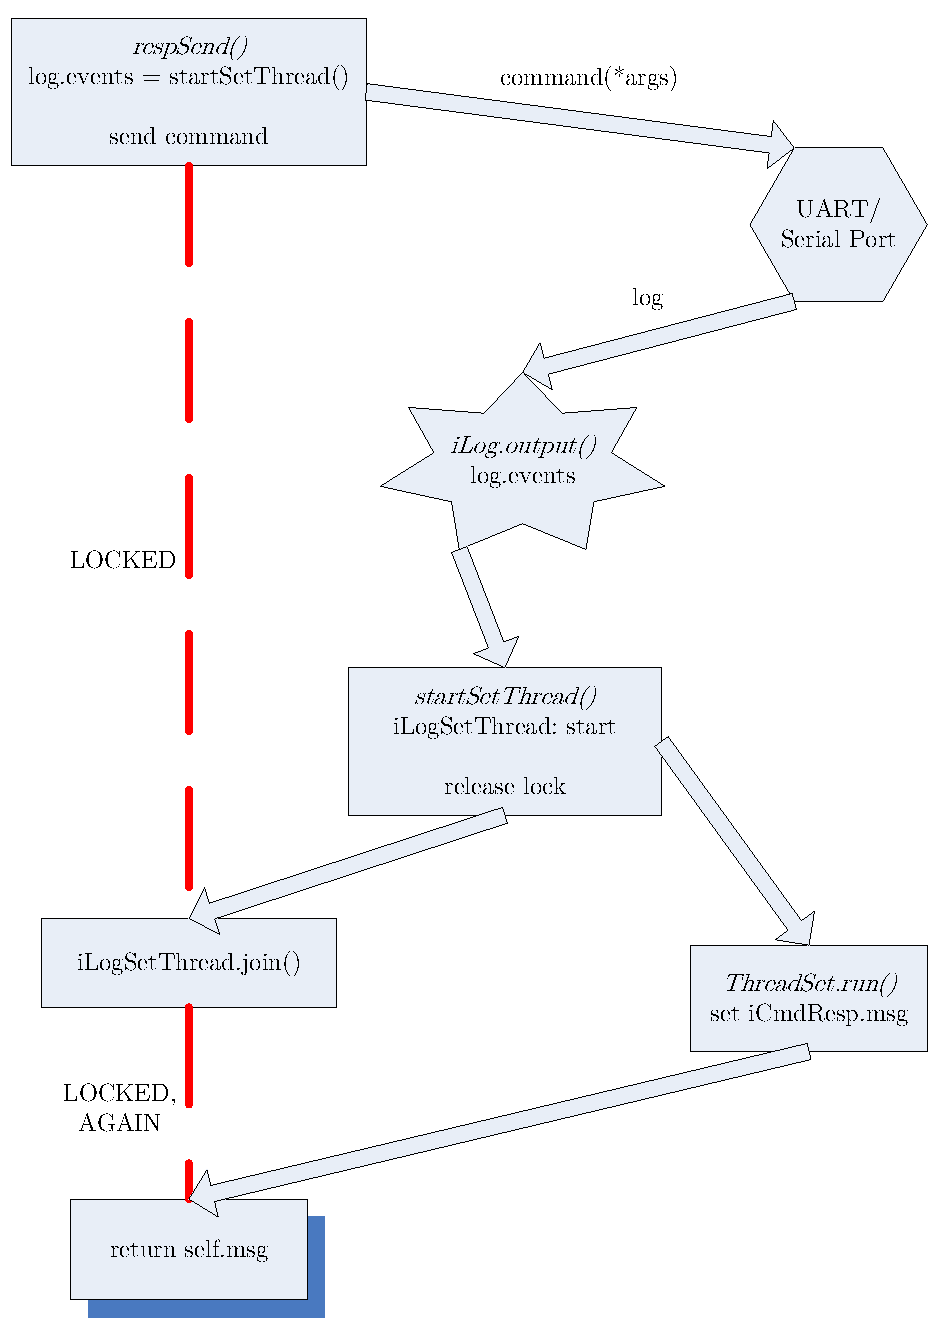
\includegraphics[scale=1]{hobbes_icmdresp.pdf}
\end{center}

\setcounter{subsubsection}{-1}



%
% Section 4.7.0
%
\subsubsection{Classes}
\label{4.7.0}

\setcounter{paragraph}{-1}



%
% Section 4.7.0.0
%
\paragraph{iCmdResp}
\label{4.7.0.0}

Contains the iCommand and iLog to work with, and a function to send the iCommand and wait for an appropriate iLog.



%
% Section 4.7.0.1
%
\paragraph{ThreadSet}
\label{4.7.0.1}

Extends the Python \href{http://docs.python.org/library/threading.html#thread-objects}{Thread} class to set the message of an iCmdResp, which is eventually returned at the end of respSend().



%
% Section 4.7.1
%
\subsubsection{Functions}
\label{4.7.1}

\setcounter{paragraph}{-1}



%
% Section 4.7.1.0
%
\paragraph{iCmdResp}
\label{4.7.1.0}

Functions in the iCmdResp class:

\setcounter{subparagraph}{-1}



%
% Section 4.7.1.0.0
%
\subparagraph{\_\_init\_\_()}
\label{4.7.1.0.0}

\emph{Arguments:} self; line - the line from an ``icmdresp'' file to parse; componentName - the name of the iComponent containing the iCommand and iLog to be set; device - the Device containing the iCmdResp object

\emph{Returns:} None

This function does the following:

\begin{enumerate}

\item Parses line, which looks like ``R:[response] C:[command] L:[log] A:[arg]'', to get the response name, iCommand name, iLog name, and iLog argument index.

\item Find and save references to the iCommand and iLog of the iCmdResp.

\item Saves a reference to device, as it will be used later.

\item Creates a Python \href{http://docs.python.org/library/threading.html#lock-objects}{Lock} instance and calls acquire() once. This means that the next thread that calls acquire() will be locked until release() is called in a different thread.

\end{enumerate}



%
% Section 4.7.1.0.1
%
\subparagraph{respSend()}
\label{4.7.1.0.1}

\emph{Arguments:} self; *args - a tuple of iCommand arguments

\emph{Returns:} None

Looking at the preceding diagram may help.

\begin{enumerate}

\item Saves the current events of the iLog. They will be restored at the end.

\item Set the new event handler of the iLog as \hyperref[4.7.1.0.2]{startSetThread()}.

\item Send the iCommand with *args as the arguments.

\item Acquire the lock, locking this thread.  respSend will attempt to acquire the lock for 3 seconds before giving up and returning None. This timeout should be sufficiently long enough to only occur if the device has been disconnected.

\item Join \hyperref[4.7.2.4.7]{iLogSetThread}, locking this thread again.

\item Restore the original event handler(s) of the iLog.

\item Return the \hyperref[4.7.2.4.8]{self.msg} variable.

\end{enumerate}



%
% Section 4.7.1.0.2
%
\subparagraph{startSetThread()}
\label{4.7.1.0.2}

\emph{Arguments:} self; sender - the iLog causing this function to be called; args

\emph{Returns:} None

Creates a thread that will set the iCmdResp's message.

\emph{Is this really necessary?} Maybe. The whole module would be much easier to comprehend if a thread wasn't created here, but .NET and its event handling is iffy. If it ever turns out that code execution and iLog parsing occur on the same thread, you have an instant deadlock.

\begin{enumerate}

\item Saves the sender argument, i.e. the iLog.

\item Creates a ThreadSet instance. Note that in order to save the iCmdResp in this instance, self is passed in as an argument.

\item Starts the newly-created ThreadSet instance.

\item Release the lock so \hyperref[4.7.1.0.1]{respSend()} can then unlock (only to lock again, of course).

\end{enumerate}



%
% Section 4.7.1.1
%
\paragraph{ThreadSet}
\label{4.7.1.1}

Functions in the ThreadSet class:

\setcounter{subparagraph}{-1}



%
% Section 4.7.1.1.0
%
\subparagraph{\_\_init\_\_()}
\label{4.7.1.1.0}

\emph{Arguments:} self; iCmdResp - the iCmdResp calling this function

\emph{Returns:} None

Saves the iCmdResp reference, then calls \_\_init\_\_() of the parent Thread class to initialize everything else (following proper Python conventions).



%
% Section 4.7.1.1.1
%
\subparagraph{run()}
\label{4.7.1.1.1}

\emph{Arguments:} self

\emph{Returns:} None

Called when the start() function of the underlying Thread is called. Sets the iCmdResp's message by retrieving the appropriate argument from the arguments of the appropriate iLog.



%
% Section 4.7.2
%
\subsubsection{Variables and miscellaneous}
\label{4.7.2}

Some module-level variables are included here.

\setcounter{paragraph}{-1}


%
% Section 4.7.2.0
%
\paragraph{responseSplit}
\label{4.7.2.0}

The string ``R:''. Used to parse the line argument in \_\_init\_\_().



%
% Section 4.7.2.1
%
\paragraph{commandSplit}
\label{4.7.2.1}

The string `` C:''. Used to parse the line argument in \_\_init\_\_().



%
% Section 4.7.2.2
%
\paragraph{logSplit}
\label{4.7.2.2}

The string `` L:''. Used to parse the line argument in \_\_init\_\_().



%
% Section 4.7.2.3
%
\paragraph{argSplit}
\label{4.7.2.3}

The string `` A:''. Used to parse the line argument in \_\_init\_\_().



%
% Section 4.7.2.4
%
\paragraph{iCmdResp}
\label{4.7.2.4}

Variables in the iCmdResp class:

\setcounter{subparagraph}{-1}



%
% Section 4.7.2.4.0
%
\subparagraph{response}
\label{4.7.2.4.0}

The name of the iCmdResp. This is only used when creating Python wrappers for iCmdResps.



%
% Section 4.7.2.4.1
%
\subparagraph{command}
\label{4.7.2.4.1}

The iCommand used in the iCmdResp.



%
% Section 4.7.2.4.2
%
\subparagraph{log}
\label{4.7.2.4.2}

The iLog used in the iCmdResp.



%
% Section 4.7.2.4.3
%
\subparagraph{argIndex}
\label{4.7.2.4.3}

The argument index of the iLog's argument to set as the iCmdResp's message.



%
% Section 4.7.2.4.4
%
\subparagraph{device}
\label{4.7.2.4.4}

A reference to the Device this iCmdResp is a part of.



%
% Section 4.7.2.4.5
%
\subparagraph{lock}
\label{4.7.2.4.5}

A Python Lock used for locking a thread.


%
% Section 4.7.2.4.6
%
\subparagraph{sender}
\label{4.7.2.4.6}

The iLog firing the event once it is completely parsed.



%
% Section 4.7.2.4.7
%
\subparagraph{iLogSetThread}
\label{4.7.2.4.7}

An instance of the ThreadSet class.



%
% Section 4.7.2.4.8
%
\subparagraph{msg}
\label{4.7.2.4.8}

The message of the iCmdResp to return.



%
% Section 4.7.2.5
%
\paragraph{ThreadSet}
\label{4.7.2.5}

Variables in the ThreadSet class:

\setcounter{subparagraph}{-1}



%
% Section 4.7.2.5.0
%
\subparagraph{iCmdResp}
\label{4.7.2.5.0}

The iCmdResp whose message should be set.



%
% Section 4.8
%
\subsection{Stewie}
\label{4.8}

Sends an image file to a board using the Stewie file transfer protocol.

\setcounter{subsubsection}{-1}



%
% Section 4.8.0
%
\subsubsection{Classes}
\label{4.8.0}

None.



%
% Section 4.8.1
%
\subsubsection{Functions}
\label{4.8.1}

\setcounter{paragraph}{-1}



%
% Section 4.8.1.0
%
\paragraph{sendFileByStewie()}
\label{4.8.1.0}

\emph{Arguments:} dev - the Device to send the file; name - the name of the file as specified in icron\_header

\emph{Returns:} True if transfer was successful, False otherwise

First, uses ``name'' to extract the actual binary to send. Hobbes 0 uses bsdtar.exe.

Then, checks the Stewie file to make sure the file is formatted correctly (note all bytes are represented in decimal):

\begin{itemize}

\item The header must be four bytes: 83, 48, 48, and 51.

\item The footer must be two bytes: 83 and 56.

\item Each record in the binary should contain, in order, 83, the address length, the record length, the address, the actual data, and the checksum.

\item The address length must be 49, 50, or 51. These bytes correspond to an address length of 2, 3, and 4. This length is included in the record length.

\item The record length must be at least the same value as the address length (of course), and cannot result in bytes being read past the end of the file.

\item The checksum is calculated by adding together the bytes from the record length byte to the end of the actual data (including the ends), taking the complement of the sum, then masking the result by 0xFF. This checksum must match the checksum byte located at the index directly after the data.

\end{itemize}

If any of these conditions are not satisfied, an error message should be printed and the function would return False.

If all of the conditions are satisfied, sending can begin:

\begin{itemize}

\item Send 63 (``?'') to the board. If 64 (``@'') is not received in 2 seconds, retry. If there have been 3 retries, quit the function.

\item Send the header of 83, 48, 48, and 51. If 123 (``\{'') is not received in 2 seconds, quit.

\item Send each record. If 126 (``\textasciitilde'') is not received in 2 seconds after sending, quit.

\item Send the footer of 83 and 56. If 125 (``\}'') is not received in 2 seconds, quit.

\end{itemize}

Once 125 is received, bootloading is finished and the function can return True.



%
% Section 4.8.2
%
\subsubsection{Variables and miscellaneous}
\label{4.8.2}

None. Well, there are variables, but they can easily change.



%
% Section 4.9
%
\subsection{XMODEM}
\label{4.9}

Sends an image file to a board using the XMODEM file transfer protocol.

\setcounter{subsubsection}{-1}



%
% Section 4.9.0
%
\subsubsection{Classes}
\label{4.9.0}

None.



%
% Section 4.9.1
%
\subsubsection{Functions}
\label{4.9.1}

\setcounter{paragraph}{-1}



%
% Section 4.9.1.0
%
\paragraph{sendFileByXMODEM()}
\label{4.9.1.0}

\emph{Arguments:} dev - the Device to send the file to; name - the name of the file as specified in the .icron file

\emph{Returns:} True if the file was successfully sent, False otherwise

Wait for a NAK to be received. If it isn't in 5 seconds, quit. Note that 5 seconds is required, as this function is called directly after flashing a flash writer to the board. The board must first finish erasing the flash and verifying it before becoming ready for XMODEM transfer and sending a NAK.

Untars the binary to be sent, and calls send\_XMODEM\_raw\_binary() with the result.



%
% Section 4.9.1.1
%
\paragraph{send\_XMODEM\_raw\_binary()}
\label{4.9.1.1}

\emph{Arguments:} dev - the Device to send the binary to; binary\_bytes - the bytes of the binary; file\_name - the name of the file being sent

\emph{Returns:} None

Sends the binary\_bytes variable (as some sort of collection) to the board using the XMODEM protocol:

\begin{enumerate}

\item Send a packet of 132 bytes to the board. This is composed of all bytes, so values will wrap if they go below 0 or go above 255:

\begin{itemize}

\item SOH (the byte 1)

\item The packet number, i.e. n where the packet is the nth one being sent

\item The inverse packet number: 255 - (packet number)

\item The data: 128 bytes of the binary, or the rest of the binary padded by 0xFFs to 128 bytes

\item The checksum: the sum of the data mod 256

\end{itemize}

\item After the packet is sent, wait for a response. If there is no response in 2 seconds, time out. If there is a response of an ACK (byte 6), send the next packet. If there is a response of a NAK (byte 21), try sending the packet again. Allow a maximum of 10 retries; if this maximum is reached, quit the function.

\item Finally, send an EOT (byte 4). Do the same procedure of waiting and possibly resending as if a packet had been sent.

\end{enumerate}

Lastly, notify the user transfer was successful and return True.



%
% Section 4.9.2
%
\subsubsection{Variables and miscellaneous}
\label{4.9.2}

None. Again, depends on the implementation.

The splitting of flashing a board via XMODEM into two functions means one can call send\_XMODEM\_raw\_binary() to send a binary that is not in a .icron file.



%
% Section 5
%
\section{Test Plan}
\label{5}

There shouldn't be a need for a detailed test plan. If it works, great. If it crashes, maybe there's a bug or .NET is just plain bad in the case of Hobbes 0.



\end{document}